% Options for packages loaded elsewhere
\PassOptionsToPackage{unicode}{hyperref}
\PassOptionsToPackage{hyphens}{url}
\PassOptionsToPackage{dvipsnames,svgnames,x11names}{xcolor}
%
\documentclass[
  12pt,
]{article}
\usepackage{amsmath,amssymb}
\usepackage{lmodern}
\usepackage{iftex}
\ifPDFTeX
  \usepackage[T1]{fontenc}
  \usepackage[utf8]{inputenc}
  \usepackage{textcomp} % provide euro and other symbols
\else % if luatex or xetex
  \usepackage{unicode-math}
  \defaultfontfeatures{Scale=MatchLowercase}
  \defaultfontfeatures[\rmfamily]{Ligatures=TeX,Scale=1}
\fi
% Use upquote if available, for straight quotes in verbatim environments
\IfFileExists{upquote.sty}{\usepackage{upquote}}{}
\IfFileExists{microtype.sty}{% use microtype if available
  \usepackage[]{microtype}
  \UseMicrotypeSet[protrusion]{basicmath} % disable protrusion for tt fonts
}{}
\makeatletter
\@ifundefined{KOMAClassName}{% if non-KOMA class
  \IfFileExists{parskip.sty}{%
    \usepackage{parskip}
  }{% else
    \setlength{\parindent}{0pt}
    \setlength{\parskip}{6pt plus 2pt minus 1pt}}
}{% if KOMA class
  \KOMAoptions{parskip=half}}
\makeatother
\usepackage{xcolor}
\IfFileExists{xurl.sty}{\usepackage{xurl}}{} % add URL line breaks if available
\IfFileExists{bookmark.sty}{\usepackage{bookmark}}{\usepackage{hyperref}}
\hypersetup{
  pdftitle={Winning the Startup Game},
  pdfauthor={Simão Policarpo Nogueira},
  colorlinks=true,
  linkcolor={blue},
  filecolor={Maroon},
  citecolor={Blue},
  urlcolor={Blue},
  pdfcreator={LaTeX via pandoc}}
\urlstyle{same} % disable monospaced font for URLs
\usepackage[margin=1in]{geometry}
\usepackage{longtable,booktabs,array}
\usepackage{calc} % for calculating minipage widths
% Correct order of tables after \paragraph or \subparagraph
\usepackage{etoolbox}
\makeatletter
\patchcmd\longtable{\par}{\if@noskipsec\mbox{}\fi\par}{}{}
\makeatother
% Allow footnotes in longtable head/foot
\IfFileExists{footnotehyper.sty}{\usepackage{footnotehyper}}{\usepackage{footnote}}
\makesavenoteenv{longtable}
\usepackage{graphicx}
\makeatletter
\def\maxwidth{\ifdim\Gin@nat@width>\linewidth\linewidth\else\Gin@nat@width\fi}
\def\maxheight{\ifdim\Gin@nat@height>\textheight\textheight\else\Gin@nat@height\fi}
\makeatother
% Scale images if necessary, so that they will not overflow the page
% margins by default, and it is still possible to overwrite the defaults
% using explicit options in \includegraphics[width, height, ...]{}
\setkeys{Gin}{width=\maxwidth,height=\maxheight,keepaspectratio}
% Set default figure placement to htbp
\makeatletter
\def\fps@figure{htbp}
\makeatother
\setlength{\emergencystretch}{3em} % prevent overfull lines
\providecommand{\tightlist}{%
  \setlength{\itemsep}{0pt}\setlength{\parskip}{0pt}}
\setcounter{secnumdepth}{5}
\newlength{\cslhangindent}
\setlength{\cslhangindent}{1.5em}
\newlength{\csllabelwidth}
\setlength{\csllabelwidth}{3em}
\newlength{\cslentryspacingunit} % times entry-spacing
\setlength{\cslentryspacingunit}{\parskip}
\newenvironment{CSLReferences}[2] % #1 hanging-ident, #2 entry spacing
 {% don't indent paragraphs
  \setlength{\parindent}{0pt}
  % turn on hanging indent if param 1 is 1
  \ifodd #1
  \let\oldpar\par
  \def\par{\hangindent=\cslhangindent\oldpar}
  \fi
  % set entry spacing
  \setlength{\parskip}{#2\cslentryspacingunit}
 }%
 {}
\usepackage{calc}
\newcommand{\CSLBlock}[1]{#1\hfill\break}
\newcommand{\CSLLeftMargin}[1]{\parbox[t]{\csllabelwidth}{#1}}
\newcommand{\CSLRightInline}[1]{\parbox[t]{\linewidth - \csllabelwidth}{#1}\break}
\newcommand{\CSLIndent}[1]{\hspace{\cslhangindent}#1}
\usepackage{blindtext} % for dummy text in the beta version
\usepackage{setspace} % line spacing
\usepackage{geometry} % margins, etc
\geometry{margin=2.5cm}
\usepackage{fontspec}
\setmainfont{Times New Roman}
\usepackage[nottoc]{tocbibind} % lof and lot in toc
\usepackage{caption} % captions formatting
\captionsetup{justification   = raggedright,
              singlelinecheck = false,
              format = hang,
              labelfont = bf}
\usepackage{tocloft} % lof and lot editing
\renewcommand{\cftfigfont}{Figure }
\renewcommand{\cfttabfont}{Table }
\expandafter\def\expandafter\quote\expandafter{\quote\singlespacing} %single spacing in quotes
\AtBeginDocument{\let\maketitle\relax}

\usepackage{fontspec}
\setmainfont{Times New Roman}

\usepackage{dcolumn}

% Avoid weird line and word breaks
\tolerance=1
\emergencystretch=\maxdimen
\hyphenpenalty=10000
\hbadness=10000
\usepackage{booktabs}
\usepackage{longtable}
\usepackage{array}
\usepackage{multirow}
\usepackage{wrapfig}
\usepackage{float}
\usepackage{colortbl}
\usepackage{pdflscape}
\usepackage{tabu}
\usepackage{threeparttable}
\usepackage{threeparttablex}
\usepackage[normalem]{ulem}
\usepackage{makecell}
\usepackage{xcolor}
\ifLuaTeX
  \usepackage{selnolig}  % disable illegal ligatures
\fi

\title{Winning the Startup Game}
\usepackage{etoolbox}
\makeatletter
\providecommand{\subtitle}[1]{% add subtitle to \maketitle
  \apptocmd{\@title}{\par {\large #1 \par}}{}{}
}
\makeatother
\subtitle{A Study on the Design of European Startup Accelerators}
\author{Simão Policarpo Nogueira}
\date{January 5, 2022}

\begin{document}
\maketitle

\pagenumbering{gobble}

\begin{figure}

{\centering 
\includegraphics[width=0.5\linewidth]{./writing/figures/logo_catolica} 

}

\end{figure}

\begin{centering}
\vfill
\begin{spacing}{1}
{\Huge\bf Winning the Startup Game}\\
\vspace{1em}
\parbox{28em}{\centering\Huge A Study on the Design of European Startup Accelerators}
\end{spacing}
\vfill 
{\LARGE\bf Simão Policarpo Nogueira}
\vfill 
\parbox{25em}{\centering\Large Dissertation written under the supervision of Professor José Vasconcelos-Sousa.} 
\vfill 
\parbox{38em}{\centering\Large Dissertation submitted in partial fulfilment of requirements for the MSc in Business, at the Universidade Católica Portuguesa, January 5, 2022.}

\end{centering}
\clearpage
\pagenumbering{roman}
\setstretch{1.5}

\clearpage

\hypertarget{acknowledgments}{%
\section*{Acknowledgments}\label{acknowledgments}}
\addcontentsline{toc}{section}{Acknowledgments}

Many are those who I wish to thank and acknowledge. It is to you I dedicate the many hours of work behind this document.

Firstly, to my advisor, Professor José Vasconcelos-Sousa, whose guidance, expertise and round-the-clock availability successfully portray what I have excitedly experienced at CATÓLICA-LISBON for the duration of my Master's program. Your honest enthusiasm for the topic and belief in my success from the very beginning were imperative for the writing of this dissertation.

To Nest Collective and our team, for the trust and confidence in the effort I placed on this research and for reviewing my work. You have allowed me to grow personally and professionally from the very beginning of my career. This has been my second - almost first! - home for the last years and will hopefully be so for many more.

To Crunchbase, for allowing access to their data without which I would not have been able to complete my analysis but also for their contributions to the scientific community that I am sure have generated numerous, impactful studies.

And lastly, to those who stand with me no matter what - here and someplace else. To my family, to my friends, to my girlfriend, Rafa, for your support, patience and love. Never have I felt alone.

\clearpage

\hypertarget{abstract}{%
\section*{Abstract}\label{abstract}}
\addcontentsline{toc}{section}{Abstract}

\textbf{Title:} Winning the Startup Game: A Study on the Design of European Startup Accelerators\\
\textbf{Author:} Simão Policarpo Nogueira\\
\textbf{Keywords:} Incubators; Accelerators; Startups; Entrepreneurship; Innovation.

~

The European startup and investment scene is quickly expanding: record levels of growth were identified in 2021, revealing this region lacks only in maturity of the ecosystem. Startup accelerators - the new generation of incubators - have picked up on this expansion and turned acceleration into a successful venture. As researchers continue to disagree on the conceptual and typological definitions of startup accelerators, their impact and ideal structure remain unclear. This dissertation aims to transpose a study conducted in the USA startup ecosystem to the European reality through intensive use of data and statistics. It looks into the relationships between the design variables of acceleration programs and the success - or lack thereof - of their graduated startups. Data was collected through a range of aggregators, news articles and websites and put through linear regression models in order to test the hypothesis that an accelerator's structure impacts its startup's chances of success. Our results reflect the positive effects of a large and diversified network of partners, sponsors, founders, and companies but struggled to explain the mechanisms behind startup success in full. Our data allowed us to distinguish between ill- and well-designed accelerators, establishing that the impact of the latter is stronger in both the short- and long-term, ultimately proposing the structure for an accelerator that maximises a startup's chances of success.

\clearpage

\hypertarget{resumo}{%
\section*{Resumo}\label{resumo}}
\addcontentsline{toc}{section}{Resumo}

\textbf{Title:} Winning the Startup Game: A Study on the Design of European Startup Accelerators\\
\textbf{Author:} Simão Policarpo Nogueira\\
\textbf{Palavras-chave:} Incubadoras; Aceleradoras; Startups; Empreendedorismo; Inovação.

~

O panorama Europeu de startups e investimento tem vindo a desenvolver-se rapidamente: identificaram-se níveis recorde de crescimento em 2021, revelando que o ecossistema carece apenas de maturidade. As aceleradoras de startups - a nova geração de incubadoras -, lado-a-lado com esta expansão, tornaram a aceleração num negócio de sucesso. Da mesma forma que a investigação continua a discordar sobre as suas definições conceptuais e tipológicas, o impacto e a estrutura ideal das aceleradoras permanecem pouco claros. Esta dissertação visa transpor um estudo realizado no ecossistema dos EUA para a realidade Europeia através da utilização de dados e estatística, ao analisar as relações entre as variáveis que compõem os programas de aceleração e o sucesso - ou falta dele - das startups que os completam. Os dados foram recolhidos através de uma série de agregadores, notícias e websites, e inseridos em modelos de regressão linear a fim de testar a hipótese de que a estrutura de uma aceleradora tem impacto na probabilidade de sucesso das suas startups. Os nossos resultados reflectem os efeitos positivos de uma grande e diversificada rede de parceiros, patrocinadores, fundadores e empresas, mas tiveram dificuldade em explicar na íntegra os mecanismos por detrás do sucesso da aceleração. Os nossos dados permitiram distinguir entre aceleradoras mal e bem concebidas, estabelecendo que o impacto das segundas é mais forte tanto a curto quanto a longo prazo, dando lugar à proposta de uma estrutura para uma aceleradora que maximiza as hipóteses de sucesso das startups.

\clearpage{\hypersetup{linkcolor=black}\tableofcontents}
\clearpage{\hypersetup{linkcolor=black}\listoffigures\listoftables}
\clearpage\pagenumbering{arabic}\setcounter{page}{1}

\clearpage

\hypertarget{introduction}{%
\section{Introduction}\label{introduction}}

\hypertarget{the-european-ecosystem-its-startups-and-accelerators}{%
\subsection{The European Ecosystem, Its Startups, and Accelerators}\label{the-european-ecosystem-its-startups-and-accelerators}}

Startups fail - a lot. As many as 9 out of every 10 will not accomplish the goals they set out to achieve (\protect\hyperlink{ref-nobel_companies_2011}{Nobel 2011}). Understanding the mechanisms behind failure is necessarily relevant, but so is finding strategies to combat this lack of success and accelerate innovation in a range of ecosystems. Entrepreneurs, managers, venture capitalists, and policymakers have long pursued this target (\protect\hyperlink{ref-barbero_different_2014}{Barbero et al. 2014}; \protect\hyperlink{ref-colombelli_be_2016}{Colombelli, Krafft, and Vivarelli 2016}) and have found business incubators and similar vehicles to be ideal facilitators for the early-stage development of startups (\protect\hyperlink{ref-hackett_systematic_2004}{Hackett and Dilts 2004}) and as a source of sustainable value creation (\protect\hyperlink{ref-colombelli_be_2016}{Colombelli, Krafft, and Vivarelli 2016}).

Moreover, the exponential growth in the number of startup accelerators and incubators in recent years and the ever-changing founder and company needs have created opportunities for researchers who now try to understand these phenomena. Nevertheless, ``startups at the youngest stages of development have long been invisible to researchers'' (\protect\hyperlink{ref-cohen_design_2019}{Cohen et al. 2019}). With this in mind, current literature discloses three areas of interest surrounding startup accelerators as a subset of startup incubators, namely on their definitions and typologies, on the process which the cohort goes through, and on the performance and impact of the programs (\protect\hyperlink{ref-hausberg_business_2020}{Hausberg and Korreck 2020}).

Europe reached record levels of growth and investment in 2021. ``With a record \$100B of capital invested, 98 new unicorns, and the strongest ever startup pipeline'', the European region is comparable with the United States of America (USA) in many metrics, only lacking behind in ecosystem maturity (\protect\hyperlink{ref-european_tech_2021}{State of European Tech 2021}).

This dissertation will uncover how the different components that make up a European acceleration program play a part in the success of young startups, following the steps of research conducted in the USA that has shown ``clear patterns of association between design choices and (startup) performance'' (\protect\hyperlink{ref-cohen_design_2019}{Cohen et al. 2019}). Through a collection of data points over a large number of accelerators and startups in the region, quantitative statistical analysis with regression models was conducted, paving the way to understand existing correlation mechanisms and relationships between program design variables and company performance metrics. This wealth of data is, in turn, converted into a broad definition of ill- and well-designed accelerator. The resulting evidence allows managers to make informed decisions on how to structure an incubator's acceleration program and proves - to a certain extent - that accelerators impact the success of incubated startups.

\hypertarget{researcher-background}{%
\subsection{Researcher Background}\label{researcher-background}}

Portugal is often referred to as the Silicon Valley of Europe (\protect\hyperlink{ref-dinheiro_vivo_2019}{dinheiro vivo 2019}). The year-round good weather, ecosystem, and hospitality make it a breeding ground for promising startups which, every year, meet at Web Summit to share knowledge and experience the comparably pleasant Night Summit. The writer of this dissertation currently heads operations at \href{https://nestcollective.co}{Nest Collective}, a collective of digital product studios with a distinct model for company collaboration and incubation in the central region of the country. Having been part of the entrepreneurial ecosystem for the last quarter of their life, their perception of the growth potential for business incubators was made clear by their participation in several student-run organizations, software, and design consulting agencies and startups.

Questioning themselves as to what could be the next strategic step for the incubator, the generational timeline proposed by Bruneel et al. (\protect\hyperlink{ref-bruneel_evolution_2012}{2012}) prompted the author to consider startup acceleration as Nest Collective's next endeavour. Understanding ``innovative ventures exhibit higher survival rates'' and that certain ``circumstances that facilitate the formation of innovative start-ups and the survival of young innovative firms'' (\protect\hyperlink{ref-colombelli_be_2016}{Colombelli, Krafft, and Vivarelli 2016}) may be - to a certain extent - the responsibility of managers and directors of these ecosystems, the author proposes a study which has the opportunity of assisting them and others in making data-backed decisions for more successful acceleration programs and, in consequence, higher-achieving startups with reduced failure rates.

\hypertarget{problem-statement}{%
\subsection{Problem Statement}\label{problem-statement}}

With the end goal of suggesting a set of managerial and theoretical implications, the aim of this thesis is twofold: firstly, to understand the impact of a European acceleration program's design features on the success metrics of its accelerated startups, and, secondly, to propose and verify a data-based definition of well- and ill-designed accelerator. The problem statement can be defined as: The impact of startup accelerator program design variables in a graduated startup's chance of success in the European context.

In answering the above problem statement, two research questions and corresponding hypotheses for testing were crafted and analyzed under quantitative, statistical models. The research questions (RQ) are:

\begin{itemize}
\item
  RQ1: Do accelerator program design variables affect a graduated startup's chance of success?
\item
  RQ2: Are there performance differences between startups who graduated from ill- and well-designed accelerator programs?
\end{itemize}

\clearpage

\hypertarget{literature-review}{%
\section{\texorpdfstring{\emph{Accelewho}?: A Literature Review}{Accelewho?: A Literature Review}}\label{literature-review}}

The concept of startup is just as sexy as it is complex - perhaps not the designation itself, but what it encompasses and how the media has portrayed it for as long as there have been garages in Silicon Valley. With the advent of technology, collaboration is not only easier but comes as a requirement for innovation and relevancy in an ever-evolving business world. Joint effort cooperation resulting from the systemic interaction between companies, investors, and other stakeholders - the Entrepreneurial Ecosystem -, paved the way for what we now know as startup incubators and trickled down to more structured incubation programs: startup accelerators. This dissertation and research efforts will focus on the structural elements of an acceleration program and how they impact and influence the outcome of graduated startups.

\hypertarget{defining-startup-incubator}{%
\subsection{Defining Startup Incubator}\label{defining-startup-incubator}}

The incubator phenomenon has its roots in New York, 1959 (\protect\hyperlink{ref-lewis_does_2002}{Lewis 2002}). Whereas nowadays entrepreneurs willingly build and design spaces to host multiple companies, the owner of this first incubator did it out of necessity: ``Unable to find a tenant capable of leasing the entire facility, the developer opted to sublet subdivided partitions of the building'' (\protect\hyperlink{ref-hackett_systematic_2004}{Hackett and Dilts 2004}). From thereon-out, the akin needs of the renting companies in terms of accounting, legal and other basic business support services made it so that this model could prove its relevancy and scale, finding slow growth in the 1960s and 1970s (\protect\hyperlink{ref-hackett_systematic_2004}{Hackett and Dilts 2004}). With the help of regulatory entities in the US that ``recognized the importance of innovation and intellectual property rights protection'' (\protect\hyperlink{ref-hackett_systematic_2004}{Hackett and Dilts 2004}), the onset of academic and non-academic research being conducted on the same topic provided the right environment for a larger increase in the number of operating incubators in the 1980s. Still before the turn of the century (in the 1990s), hand-in-hand with the expansion of online business firms, startup incubators were the personification of the dream and romanticizing of Entrepreneurship and the Rockstar Entrepreneur. Even with the downfall of the global economy after the US stock market bubble in 2008, startup incubators still play a large role in the modern entrepreneurial ecosystem and economy (\protect\hyperlink{ref-hackett_systematic_2004}{Hackett and Dilts 2004}; \protect\hyperlink{ref-hausberg_business_2020}{Hausberg and Korreck 2020}). A further step in understanding startup accelerators is defining what precedes it: the incubator.

\begin{quote}
The incubator is ``an enterprise that facilitates the early-stage development of firms by providing office space, shared services, and business assistance.''

(\protect\hyperlink{ref-hackett_systematic_2004}{Hackett and Dilts 2004})
\end{quote}

~

\hypertarget{typology-of-startup-incubators}{%
\subsection{Typology of Startup Incubators}\label{typology-of-startup-incubators}}

An area of research commonly approached by authors is the conceptual study of incubators and accelerators: for Hochberg, the ``conceptual description of the accelerator model'' and for Hackett and Dilts, ``incubator configurations'' (\protect\hyperlink{ref-hochberg_accelerating_2016}{Hochberg 2016}; \protect\hyperlink{ref-hackett_systematic_2004}{Hackett and Dilts 2004}). Understanding the underlying characteristics of an incubator may provide information on its accelerator programs' potential outcomes. Hausberg and Korreck (\protect\hyperlink{ref-hausberg_business_2020}{2020}) conducted a co-citation analysis of literature, building on previous theories surrounding incubators and accelerators such as that of Hochberg (\protect\hyperlink{ref-hochberg_accelerating_2016}{2016}) and the one proposed by Hackett and Dilts (\protect\hyperlink{ref-hackett_systematic_2004}{2004}). Ultimately, Hausberg and Korreck (\protect\hyperlink{ref-hausberg_business_2020}{2020}) suggest a typological classification model of their own and identify the following research fields:

\begin{quote}
``(1) studies on origins, definitions, and typologies of incubators, (2) studies on the incubation process, and (3) studies on impact and performance.''

(\protect\hyperlink{ref-hausberg_business_2020}{Hausberg and Korreck 2020})
\end{quote}

~

The authors also make the case that research on the first stream makes up a relevant share of available literature, therefore arguing for its contextual importance. In their study, work from other authors is grouped according to the foundation upon which their classification system lies. Since we are looking into the relationship between an accelerator program and its impact on a startup, the typological analysis should refer to the support strategy and reflect a focus on the incubatee (as in, the startup) -- two of the groups Hausberg and Korreck (\protect\hyperlink{ref-hausberg_business_2020}{2020}) mention in their research.

The fast growth in the number of corporate incubators signals the need for further classification as intrapreneurship efforts do not fit into the pre-established categories. Moreover, the current belief that innovation is a requirement for sustained competitive advantage has fostered the startup culture inside larger, more established firms through the so-called intrapreneurship. These corporate incubators could be easily classified as for-profit, but this over-simplification would go against the often unclear financial benefits of these efforts and provides an opposing view to the inclusion of university-based incubators as a category - being that these are mainly non-profit but, in certain cases, through licensing of patented research and development, reap monetary benefits (\protect\hyperlink{ref-becker_corporate_2006}{Becker and Gassmann 2006}; \protect\hyperlink{ref-shankar_accelerating_2019}{Shankar and Shepherd 2019}).

\begin{quote}
``In a corporate incubator the intentions and goals are aligned to the corporation's technology focus and time frame, meanwhile in university incubators these should be linked to how the university positions itself and what role the incubator plays within the university.''

(\protect\hyperlink{ref-becker_corporate_2006}{Becker and Gassmann 2006})
\end{quote}

~

From an historical point of view, the classification of incubators and their typology has also been analysed. Beginning with the first incubator in New York, Bruneel et al. (\protect\hyperlink{ref-bruneel_evolution_2012}{2012}) divide the lifespan of company incubation into three generations. The first-generation offered ``office space and shared resources'' in the form of reception, parking space and meeting rooms. The second-generation is characterised by the efforts placed in ``coaching and training support'' for incubated firms, with shared business support services in the fields of accounting, legal and marketing. Some of these second-generation incubators already met certain criteria used to define the one followed by it - some provide coaching in the form of training sessions and workshops -, but it is in the third-generation that knowledge transfer is most valued and where ``access to technological, professional, and financial networks'' becomes the norm.

This dissertation will focus mainly on third-generation incubators due to their contemporary nature but will make no efforts to avoid any of the previously mentioned financial support mechanisms. We intend to remain open to broader definitions of both incubator and accelerator to ensure the coverage of all available programs. Having found a definition of incubator, we now move to construe the concept of startup accelerator in the following chapter.

\hypertarget{defining-startup-accelerator}{%
\subsection{Defining Startup Accelerator}\label{defining-startup-accelerator}}

\hypertarget{a-brief-history-of-accelerators}{%
\subsubsection{A Brief History of Accelerators}\label{a-brief-history-of-accelerators}}

With the industry founding pioneers \href{https://www.ycombinator.com}{Y Combinator} and \href{https://www.techstars.com}{Techstars} originating in 2005 and 2007\footnote{Fishback et al provide an earlier example of accelerator: \href{https://thefoundry.com}{The Foundry}, a medical device R\&D and development firm founded in 1998 (\protect\hyperlink{ref-fishback_finding_2007}{Fishback et al. 2007}). Although The Foundry's model is similar to that of an accelerator as depicted in this dissertation, the program's structure does not respect this definition in full. Accelerators are typically short, fixed-term programs whereas in this case, the limits of these and other accelerator program variables are not well defined.}, respectively, if the 1959's incubator birth is still a recent phenomenon, it is fair to assume a lot of research is still required for accelerators (\protect\hyperlink{ref-cohen_how_2013}{Cohen 2013}; \protect\hyperlink{ref-cohen_accelerating_2014}{Cohen and Hochberg 2014}; \protect\hyperlink{ref-cohen_design_2019}{Cohen et al. 2019}). The growth and proliferation of accelerators to over 2000 programs in 6 continents paired with the diversification to several industries has made it difficult to achieve a consensus in its conceptual definition. The impact of accelerators has also been the target of research but, due to a lack of available data, publications on this matter are scarce (\protect\hyperlink{ref-cohen_accelerating_2014}{Cohen and Hochberg 2014}). Nonetheless, it is widely accepted that accelerators are capable of increasing the size of a new venture's network, helping with branding and legitimizing their operation from its early days (\protect\hyperlink{ref-bruneel_evolution_2012}{Bruneel et al. 2012}; \protect\hyperlink{ref-wise_impact_2014}{Wise and Valliere 2014}).

\hypertarget{setting-a-clear-definition}{%
\subsubsection{Setting a Clear Definition}\label{setting-a-clear-definition}}

While ``the definition of accelerator programs remains discordant'' (\protect\hyperlink{ref-cohen_accelerating_2014}{Cohen and Hochberg 2014}), taking the first step with a metaphor similar to that of the chicken and egg - which came first? - can assist in deterministically distancing an incubator from an accelerator. Both historically and in the currently accepted typology, the incubator came before the accelerator - the latter being a subset of the first. Bruneel et al. (\protect\hyperlink{ref-bruneel_evolution_2012}{2012}) identify three generations of incubators with the third focusing mainly on providing access to networks of knowledge, resources, and contributing to the legitimacy of incubated firms. The first two generations took to a more direct interpretation of the definition of incubator, targeting real estate and intangible asset provisioning. Newer research conducted by Pauwels et al. (\protect\hyperlink{ref-pauwels_understanding_2016}{2016}) agrees with the aforementioned statements, identifying startup accelerators as ``a new generation incubation model''. Likewise, the trend in research appears to be in line with both authors and provides grounds for the interpretation used in this dissertation, bringing us closer to a definition of the term. Nonetheless, researchers remain entangled in trying to find a standardised definition for accelerators. Not only are both terms (incubator and accelerator) sometimes used as synonyms (\protect\hyperlink{ref-hausberg_business_2020}{Hausberg and Korreck 2020}), this challenge also comes from their conceptual ambiguity and the fact that programs themselves adapt to the needs of a certain ecosystem and its stakeholders (\protect\hyperlink{ref-cohen_design_2019}{Cohen et al. 2019}).

What then is the definition of a startup accelerator? These programs are an activity promoted and organized within an incubator and not the institution that incubators have become. Accelerator programs and startup ecosystems have been shown to impact the process of idea validation (\protect\hyperlink{ref-tripathi_startup_2019}{Tripathi, Oivo, et al. 2019}), a contributing factor to the success or failure of startups (\protect\hyperlink{ref-nobel_companies_2011}{Nobel 2011}). The faster an idea can be tested, the better. Accelerators assist recent firms in their product-market fit, customer segmentation, and resource procurement. They can be defined by their characteristic design elements - the ones which distinguish them from similar programs: limited duration, a specific number of participating startups (\protect\hyperlink{ref-cohen_how_2013}{Cohen 2013}), and a graduation event (\protect\hyperlink{ref-cohen_design_2019}{Cohen et al. 2019}).

\begin{quote}
The accelerator is ``a fixed-term, cohort-based program, including mentorship and educational components, that culminates in a public pitch event or demo day.''

(\protect\hyperlink{ref-cohen_accelerating_2014}{Cohen and Hochberg 2014})
\end{quote}

~

Some researchers point out that this definition should include another key element: accelerators ``provide equity funds in addition to the space, networks and mentorship'' (\protect\hyperlink{ref-wise_impact_2014}{Wise and Valliere 2014}). A choice was made to not include this variable in our definition because not all accelerator business models under the umbrella of this study provide the same equity funding mechanism. Additionally, even though Cohen and Hochberg (\protect\hyperlink{ref-cohen_accelerating_2014}{2014}) state that ``most accelerators take equity stakes in participating firms'', their decision to not include this topic in their accepted definition provides confidence in this judgment.

\hypertarget{measuring-an-accelerators-impact-on-startups}{%
\subsection{Measuring an Accelerator's Impact on Startups}\label{measuring-an-accelerators-impact-on-startups}}

\hypertarget{reviewmanagementimpact}{%
\subsubsection{Accelerator Management's Impact on the Startup}\label{reviewmanagementimpact}}

One factor which deeply contributes to understanding an accelerator's impact on a startup is its management. It is their responsibility to decide on the incubator's strategy and in turn determine which projects and startups become part of the cohort. Therefore, performance can only be as good as the management itself (\protect\hyperlink{ref-tripathi_insights_2019}{Tripathi, Seppänen, et al. 2019}). Moreover, having previously identified networking as the primary focus of third-generation incubators - the category which fits accelerators -, the management's ability to mobilize resources, build this network and manage relationships with other stakeholders (like investors, venture capitalists, and business angels) should have a direct impact on the outcome of startups.

~

\onehalfspacing





\begin{table}[H]

\caption{\label{tab:programvars}Accelerator Program Design Variables.}
\centering
\fontsize{9}{11}\selectfont
\begin{tabu} to \linewidth {>{\raggedright}X>{\raggedright\arraybackslash}p{35em}}
\toprule
Variable Name & Description\\
\midrule
Cohort & The group of startups which participates at one time in the acceleration program, chosen according to some criteria.\\
\addlinespace
Funding and equity & As in funding provided to startups and equity taken by the accelerator as means of payment for the provided services and mentorship.\\
\addlinespace
Mentorship & “A key component of many accelerator programs” (\protect\hyperlink{ref-cohen_design_2019}{Cohen et al. 2019}) and, alongside the corresponding network, a central piece to third-generation incubators.\\
\addlinespace
Formal education & A structured program made up of workshops, talks, and mentorship with industry experts and partners that all startups must go through to achieve a knowledge baseline.\\
\addlinespace
Workspace & One of the earliest forms of incubation (\protect\hyperlink{ref-hackett_systematic_2004}{Hackett and Dilts 2004}) and a source of “social and cultural impact of the program” (\protect\hyperlink{ref-cohen_design_2019}{Cohen et al. 2019}).\\
\addlinespace
Length of program and graduation event & The length of the acceleration is adapted to the cohort composition and changes according to all other design variables. This graduation event often referred to as demo day, is a showcasing opportunity for startups looking for investment and taking their first steps after an intensive program.\\
\addlinespace
Founder and managing director backgrounds and sponsors & Internal and external stakeholders whose presence and involvement add value to the program. These are usually expected to provide mentorship and, in the case of founders and managers, decide on the acceptance criteria for startups.\\
\bottomrule
\end{tabu}
\end{table}

\setstretch{1.5}

\hypertarget{review-design-elements}{%
\subsubsection{Accelerator Program Design Elements Impact on the Startup}\label{review-design-elements}}

Very early on in our research, we looked at ways to identify the most relevant publications surrounding incubation and acceleration. Taking advantage of the \href{https://scholar.google.com/}{Google Scholar} search engine, we began by analyzing all top publications under the ``Business, Economics \& Management'' category and the ``Entrepreneurship \& Innovation'' sub-category. Sorting by the h5-index (\protect\hyperlink{ref-hirsch_index_2005}{Hirsch 2005}), among others, we came across the \href{https://www.journals.elsevier.com/research-policy}{Research Policy journal}, classified as number one with h = 95.

The paper ``The design of startup accelerators'' co-written by Cohen, Fehder, Hochberg, and Murray, published in 2019 by the Research Policy journal, has been cited 103 times. It not only studies the core features of an accelerator program (Table \ref{tab:programvars}) by researching the USA ecosystem but also provides a well-structured statistical, quantitative analysis method that inspired reproduction for the European context. The method chosen by this group of researchers inspired the one used for this dissertation as they, like us, ``seek to explore and act upon the impact of accelerators'' (\protect\hyperlink{ref-cohen_design_2019}{Cohen et al. 2019}).

\hypertarget{final-overview}{%
\subsubsection{Final Overview}\label{final-overview}}

For the writing of this literature review, we analysed 18 papers, 15 of which are peer-reviewed. There's not a lot of research surrounding this topic, but the large majority accepts there is some form of impact of an accelerator on its cohort of startups (\protect\hyperlink{ref-cohen_how_2013}{Cohen 2013}; \protect\hyperlink{ref-pauwels_understanding_2016}{Pauwels et al. 2016}; \protect\hyperlink{ref-hausberg_business_2020}{Hausberg and Korreck 2020}). A study by Hallen, Cohen, and Bingham (\protect\hyperlink{ref-hallen_accelerators_2020}{2020}) reveals that startups who take part in acceleration programs are more likely to achieve significant funding and growth. This statement is especially relevant when the same remains true comparing graduated startups to those not accepted into these programs. Cohen et al. (\protect\hyperlink{ref-cohen_design_2019}{2019}) identify ``muted or even negative impacts of accelerators on startups'' in their research. These authors list two papers whose results indicate these effects. As much as that may be the case for certain scenarios, further analysis of Gonzalez-Uribe and Leatherbee (\protect\hyperlink{ref-gonzalez_effects_2018}{2018}) studies on Start-Up Chile's ecosystem reveal that, even though the basic accelerator services (cash or equity and co-working space) do not put forward any improvements for startup success, the provided educational programs - a characteristic of third-generation incubators - did in fact show ``significant increases in venture fundraising and scale''. Additionally, although statistical results in Yu (\protect\hyperlink{ref-yu_accelerators_2020}{2020}) show ``the odds of going out of business for accelerator companies over non-accelerator companies are 150\% higher'', they hypothesise that accelerators might help reduce success unpredictability for startups, leading them to close sooner rather than continue operating without a market fit or at a loss. The underlying complexity surrounding terminology may be a contributing factor to the different perspectives taken on this same matter.

Still, in line with the present-day data shortage on accelerated startups' results, it makes no sense to rule out the hypothesis that these null or negative impacts do not exist. An alternative is then to look at other mechanisms which may be responsible for the positive outcome of startups participating in acceleration programs. Hallen, Cohen, and Bingham (\protect\hyperlink{ref-hallen_accelerators_2020}{2020}) put forward the possibility of sorting and signalling. The sorting mechanism is suggested as the match between two partners which together maximize each other's value capturing. This situation leaves ``less-desirable partners to partner with others who are also less desirable'' (\protect\hyperlink{ref-hallen_accelerators_2020}{Hallen, Cohen, and Bingham 2020}). The impact exists but does not come solely from the accelerator's design features: it is due to some pre-existing condition of the startup. The case being made for signalling is on the impact of the accelerator's connections to other partners (ones part of the entrepreneurial ecosystem, such as investors and other companies). These associations may serve as signals to other interested parties and act as ``information pipes that efficiently disseminate information about a venture's quality'' (\protect\hyperlink{ref-hallen_accelerators_2020}{Hallen, Cohen, and Bingham 2020}). Nonetheless, as previously identified, third-generation incubators focus particularly on networking and its value for a startup's development. All in all, even if not particularly straightforward, the value-creating relationship between accelerator and startup is apparent in all literature.

\clearpage

\hypertarget{research-methodology}{%
\section{Research Methodology}\label{research-methodology}}

In the first two chapters of this dissertation, we established the status quo of startup acceleration and gave a brief overview of a study conducted by Cohen et al. (\protect\hyperlink{ref-cohen_design_2019}{2019}) on the design of startup accelerators. Their approach to research in the context of company incubation and startup accelerators inspired the methodology introduced in the following chapter. Through a quantitative, data-driven analysis, we aim to answer the previously introduced question: what sort of impact do startup accelerators have on their cohort of companies and projects?

\hypertarget{research-approach}{%
\subsection{Research Approach}\label{research-approach}}

As asserted before, even though the impact of accelerators has been the target of research, due to a lack of available data, publications on this matter are scarce (\protect\hyperlink{ref-cohen_accelerating_2014}{Cohen and Hochberg 2014}). From the very beginning of the research process, a key obstacle was in fact where to find available data for both the design elements of startup accelerators and for the success indicators of accelerated startups.

Taking clues from Cohen et al. (\protect\hyperlink{ref-cohen_design_2019}{2019}), we began by looking into \href{https://www.f6s.com/}{F6S}, an online community where founders can interact with companies, organisations, and investors. With its roots in 2012, the F6S community was founded by managers at two acceleration programs, both of which are in our database: Startupbootcamp and Springboard. Applying their knowledge of the field, this platform was built to host a range of application forms and information regarding available incubation and acceleration programs. From a humble beginning with just 130 acceleration programs, F6S currently hosts 2402 listings within this same category and reaches over 4 million users (\protect\hyperlink{ref-f6s_press_2012}{Gavin 2012}). Even though this community is certainly helpful for all startups, mentors, founders and entrepreneurs that use it, the available data was largely incomplete leading us to find alternatives.

In came \href{https://www.crunchbase.com/}{Crunchbase}, ``a prospecting platform for dealmakers who want to search less and close more'' (\protect\hyperlink{ref-crunchbase_2021}{Crunchbase 2021b}). Founded by \href{https://techcrunch.com}{TechCrunch} - an online publication with a focus on technology and the startup ecosystem - in 2007, Crunchbase is currently a standalone company still benefiting from its inherent connection to the venture building industry. Crunchbase's data is collected through a range of self-developed crowdsourcing mechanisms such as in-house data experts, partners, and other contributors. Access is limited behind a paywall - the business model for this company - and their data is verified and updated regularly, ensuring its validity. Their usage of artificial intelligence and machine learning fast-forwards the limitations associated with the process of collecting data by hand. The network effects of their large community of users that add, edit and verify information also positively influence the outlook and trust in the information they provide. Not only does Crunchbase host data on accelerators, covering some of the high-level details of the available programs, they also provide various types of information on accelerated companies, investments, founders, directors, and many others. Through contacts with the team behind their \href{https://about.crunchbase.com/partners/academic-research-access/}{Academic Research Access Program}, access to their complete Application Programming Interface (API) was granted for this research, therefore accelerating the rate at which the required datasets were completed.

As opposed to the reference study which used data available on the Seed Accelerator Rankings Project complemented by interviews with accelerators (\protect\hyperlink{ref-cohen_design_2019}{Cohen et al. 2019}), this solely analytical approach presented its challenges as data was often incomplete or missing and required dozens of hours of archival research on company pages, news, governmental and academic websites and social media.

\hypertarget{data-collection}{%
\subsection{Data Collection}\label{data-collection}}

Data collection was conducted programmatically whenever possible. Initially, for the F6S platform which does not make any APIs publicly available, a \href{https://www.python.org}{Python} web scraper was developed. This data was filtered with the type keyword ``Accelerator'' and location keyword ``Europe'', yielding a dataset with 491 accelerator programs. This dataset contained incomplete data points on ``Cohort Size'', ``Cohort Composition'', ``Program Duration'', ``Funding Provided'', ``Availability of Co-working Space'', and ``Accelerator Location'' (as part of the accelerator design variables described in Section \ref{review-design-elements}).

Having attained access to the Crunchbase Enterprise API (\protect\hyperlink{ref-crunchbase_documentation_2021}{Crunchbase 2021a}), the process for obtaining the required data progressed as follows, per the structure of this interface, available in Appendix \ref{crunchbasedocs}:

~

\begin{enumerate}
\def\labelenumi{\arabic{enumi}.}
\item
  ``Location'' data was requested from Crunchbase and filtered for ``European Union (EU)'' and ``United Kingdom'' to access its ``location\_identifiers'' (Table \ref{tab:crunchlocation}).
\item
  Organization data was requested with filters ``investor\_type'' and ``location\_identifiers'' and values ``accelerator'' and the previously identified ``location\_identifiers'' respectively, resulting in a list of accelerators and data points for analysis, as depicted in Table \ref{tab:crunchaccelerator}.
\item
  Information on founders (Table \ref{tab:crunchacceleratorfounder}) was requested for all accelerators found in step 2.
\item
  Data on investments from the accelerators returned on step 2 was requested and filtered by ``funding\_round\_investment\_type'' with values ``seed'' and ``pre\_seed''. The data points collected at this step are described in Table \ref{tab:crunchacceleratorinvestment}.
\item
  After collecting all investments from these accelerators, information on the invested companies was requested, returning the data points listed in Table \ref{tab:crunchstartup}.
\end{enumerate}

\hypertarget{data-analysis}{%
\subsection{Data Analysis}\label{data-analysis}}

All data requested from Crunchbase was exported as a JavaScript Object Notation (JSON) response, a standard method for this type of API and converted to a data format for analysis in the \href{https://www.r-project.org}{R} programming language. Further data processing was required to match the two sources (F6S and Crunchbase). Finally, to complete the dataset with the required information, additional research was conducted on a case-by-case basis, visiting accelerators and their stakeholders' websites as well as news articles and other sources of information including government agencies and data aggregators. The \href{https://web.archive.org}{Internet Archive platform} was useful for this component of the data collection as many of the accessed links for accelerators and their press releases were no longer available online.

From an initial 886 accelerators and 7429 startups, completed datasets were achieved for 216 accelerators and 4497 startups - values which are similar to those available in the reference paper by Cohen et al. (\protect\hyperlink{ref-cohen_design_2019}{2019}) that studied 146 accelerators and 5921 startups. The significant reduction in the amount of available and used information comes as a result of a large number of accelerators not disclosing their investments and therefore not providing relevant information to be considered in this study.

For the analysis and writing of results, the R programming language (\protect\hyperlink{ref-r_2020}{R Core Team 2020}) was chosen due to its statistical packages and integration with markdown in the form of R Markdown (\protect\hyperlink{ref-rmd_dynamic_2021}{Allaire et al. 2021}; \protect\hyperlink{ref-rmd_definitive_2018}{Xie, Allaire, and Grolemund 2018}; \protect\hyperlink{ref-rmd_cookbook_2020}{Xie, Dervieux, and Riederer 2020}). A similar analysis structure to that of the reference study by Cohen et al. (\protect\hyperlink{ref-cohen_design_2019}{2019}) is used to test against the hypotheses in question, through summary statistics and linear regressions. In increasing reproducibility of this research, an online version of this dissertation, data and code were made available (\url{https://masters.policarponogueira.com/}).

\clearpage

\hypertarget{analysis-of-results}{%
\section{Design Elements and Performance Indicators: An Analysis of Results}\label{analysis-of-results}}

In the previous chapter, we explained how data for 216 accelerators and 4497 startups was obtained. The following analysis describes the collected data and puts it through statistical models to present the results for the tests of hypothesis.

\hypertarget{sample-analysis}{%
\subsection{Sample Analysis}\label{sample-analysis}}

\hypertarget{accelerators}{%
\subsubsection{Accelerators}\label{accelerators}}

Our sample contains 216 accelerators distributed by 23 countries in the European region (Figure \ref{fig:accgeo}). The two countries with the largest number of accelerators - the United Kingdom and Germany - account for over 50\% of all analyzed programs, making them true hotspots for early- and seed-stage investments and interesting study objects for the purpose of this research (Table \ref{tab:accgeodist}).

\begin{figure}

{\centering 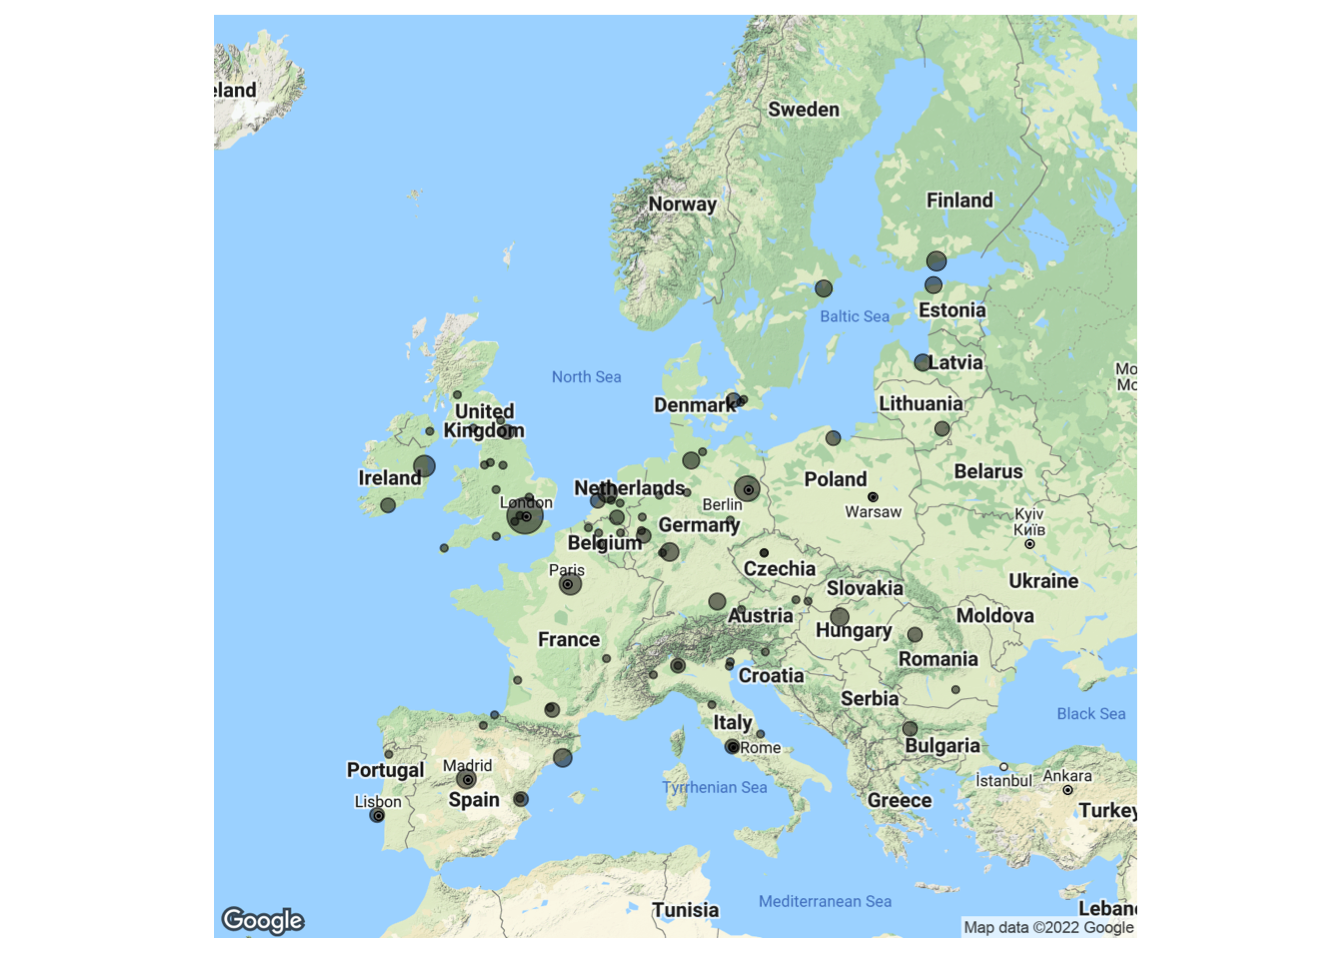
\includegraphics[width=0.95\linewidth]{winning-dissertation_files/figure-latex/accgeo-1} 

}

\caption{Accelerator Geographic Distribution.}\label{fig:accgeo}
\end{figure}

\onehalfspacing

\begin{minipage}{0.47\textwidth}
\begin{table}[H]

\caption{\label{tab:accgeodist}Accelerator Geographic Distribution.}
\centering
\fontsize{9}{11}\selectfont
\begin{tabu} to \linewidth {>{\raggedright}X>{\raggedleft}X}
\toprule
Countries & \#\\
\midrule
United Kingdom & 80\\
Germany & 33\\
Spain & 14\\
France & 13\\
The Netherlands & 12\\
\addlinespace
Italy & 11\\
Ireland & 9\\
Finland & 5\\
Sweden & 5\\
Hungary & 4\\
\addlinespace
Belgium & 3\\
Estonia & 3\\
Latvia & 3\\
Poland & 3\\
Portugal & 3\\
\addlinespace
Romania & 3\\
Austria & 2\\
Bulgaria & 2\\
Czech Republic & 2\\
Denmark & 2\\
\addlinespace
Lithuania & 2\\
Slovakia (Slovak Republic) & 1\\
Slovenia & 1\\
\bottomrule
\end{tabu}
\end{table}
\end{minipage}
\qquad
\begin{minipage}{0.47\textwidth}
\begin{table}[H]

\caption{\label{tab:addindustry}Accelerator Industry Category Variation.}
\centering
\fontsize{9}{11}\selectfont
\begin{tabu} to \linewidth {>{\raggedright}X>{\raggedleft}X}
\toprule
Industry Cluster & Percentage\\
\midrule
Financial Services & 23.102\%\\
Lending and Investments & 11.334\%\\
Professional Services & 8.731\%\\
Information Technology & 5.098\%\\
Software & 4.284\%\\
\addlinespace
Internet Services & 3.905\%\\
Education & 3.037\%\\
Science and Engineering & 2.820\%\\
Data and Analytics & 2.440\%\\
Health Care & 2.440\%\\
\addlinespace
Transportation & 2.278\%\\
Community and Lifestyle & 2.115\%\\
Media and Entertainment & 2.115\%\\
Hardware & 1.952\%\\
Commerce and Shopping & 1.518\%\\
\addlinespace
Sustainability & 1.464\%\\
Real Estate & 1.356\%\\
Artificial Intelligence & 1.193\%\\
Energy & 1.193\%\\
Sales and Marketing & 1.193\%\\
\addlinespace
Privacy and Security & 1.139\%\\
Food and Beverage & 1.030\%\\
Mobile & 1.030\%\\
All Other Clusters & 13.232\%\\
\bottomrule
\end{tabu}
\end{table}
\end{minipage}

~

~

\begin{table}[H] \centering 
  \caption{Accelerator Program Design Variables: Summary Statistics.} 
  \label{tab:accvars} 
\scriptsize 
\begin{tabular}{@{\extracolsep{1pt}}lccccc} 
\\[-1.8ex]\hline 
\hline \\[-1.8ex] 
Statistic & \multicolumn{1}{c}{N} & \multicolumn{1}{c}{Mean} & \multicolumn{1}{c}{St. Dev.} & \multicolumn{1}{c}{Min} & \multicolumn{1}{c}{Max} \\ 
\hline \\[-1.8ex] 
Cohort Size & 216 & 14.676 & 13.463 & 2 & 100 \\ 
Focused Cohort Composition & 216 & 0.546 & 0.499 & 0 & 1 \\ 
Program Duration (in number of weeks) & 216 & 19.412 & 15.127 & 0 & 144 \\ 
Funding Provided (in thousands of \$) & 216 & 66.621 & 107.259 & 0 & 1,000 \\ 
Equity Taken & 216 & 5.032 & 5.389 & 0 & 25 \\ 
Provides External Mentors & 216 & 0.792 & 0.407 & 0 & 1 \\ 
Provides Formal Education & 216 & 0.250 & 0.434 & 0 & 1 \\ 
Provides Workspace & 216 & 0.769 & 0.423 & 0 & 1 \\ 
Graduation Event & 216 & 0.866 & 0.342 & 0 & 1 \\ 
\hline \\[-1.8ex] 
\end{tabular} 
\end{table}

\setstretch{1.5}

As for accelerator industry clustering, ``Financial Services'', ``Lending and Investments'', and ``Professional Services'' make up over 43\% of the distribution. These categories represent the basic services offered by accelerators to their cohort of startups and were part of the definition of non-focused cohort compositions (which describes 54.6\% of researched programs). The most relevant focused industry clusters include ``Information Technology'', ``Software'' and ``Internet Services'' (over 13\% of the distribution). During our research, we were able to confirm this statement: a large number of the studied programs engaged with tech startups regardless of their commitment to other specific industries.

Although the percentage of accelerators that include the ``Education'' industry cluster is relatively small (\textasciitilde3\%), the percentage of those whose design choices include ``Provides Formal Education'' is much higher (25\%). This disparity brings out the challenges of defining certain aspects of acceleration programs as previously stated and following Cohen and Hochberg (\protect\hyperlink{ref-cohen_accelerating_2014}{2014}). Accelerators were found to have an average cohort size of 15 startups and a duration of 19 weeks (close to 5 months). The longest observed program ran for a full three years. Acceleration funding averaged \$66621 with 5\% equity in return for the provided services and mentorship. Most programs offered a workspace for startup teams and some form of external mentorship with their corporate, governmental, academic, or investor sponsors and stakeholders. 86.6\% of accelerators chose to showcase the work of their cohort with a final graduation event, oftentimes referred to as demo day.

There are other components that make up the design of an accelerator program, considered in Tables \ref{tab:accgeodist} to \ref{tab:accvars}: the backgrounds of founders and managing directors and the program's sponsors. In Section \ref{reviewmanagementimpact} we made the case for the importance of these stakeholders especially in the strategy and entry criteria of the program.

~

\onehalfspacing

\begin{table}[H] \centering 
  \caption{Accelerator Founding Managing Director Backgrounds: Summary Statistics.} 
  \label{tab:mdbackgroundsdesc} 
\scriptsize 
\begin{tabular}{@{\extracolsep{1pt}}lccccc} 
\\[-1.8ex]\hline 
\hline \\[-1.8ex] 
Statistic & \multicolumn{1}{c}{N} & \multicolumn{1}{c}{Mean} & \multicolumn{1}{c}{St. Dev.} & \multicolumn{1}{c}{Min} & \multicolumn{1}{c}{Max} \\ 
\hline \\[-1.8ex] 
Prior Investor Exp. & 216 & 0.088 & 0.284 & 0 & 1 \\ 
Prior Entrepreneur Exp. & 216 & 0.528 & 0.500 & 0 & 1 \\ 
Prior Corporate Exp. & 216 & 0.444 & 0.498 & 0 & 1 \\ 
Prior Academic Exp. & 216 & 0.185 & 0.389 & 0 & 1 \\ 
\hline \\[-1.8ex] 
\end{tabular} 
\end{table}

\begin{table}[H] \centering 
  \caption{Accelerator Founding Managing Director Backgrounds: Correlation.} 
  \label{tab:mdbackgroundscorr} 
\scriptsize 
\begin{tabular}{@{\extracolsep{1pt}} ccccc} 
\\[-1.8ex]\hline 
\hline \\[-1.8ex] 
 & Prior Investor Exp. & Prior Entrepreneur Exp. & Prior Corporate Exp. & Prior Academic Exp. \\ 
\hline \\[-1.8ex] 
Prior Investor Exp. &  1.000  &  &  &  \\ 
Prior Entrepreneur Exp. &  0.294\textasteriskcentered \textasteriskcentered \textasteriskcentered  &  1.000  &  &  \\ 
Prior Corporate Exp. &  0.314\textasteriskcentered \textasteriskcentered \textasteriskcentered  &  0.846\textasteriskcentered \textasteriskcentered \textasteriskcentered  &  1.000  &  \\ 
Prior Academic Exp. &  0.315\textasteriskcentered \textasteriskcentered \textasteriskcentered  &  0.451\textasteriskcentered \textasteriskcentered \textasteriskcentered  &  0.461\textasteriskcentered \textasteriskcentered \textasteriskcentered  &  1.000  \\ 
\hline \\[-1.8ex] 
\multicolumn{5}{l}{\textit{Note:} *p<0.1; **p<0.05; ***p<0.01} \\ 
\end{tabular} 
\end{table}

\setstretch{1.5}

Of all program founders and managing directors, 52.8\% were found to have experience founding other companies or organizations whereas 44.4\% had previously held a corporate job (Table \ref{tab:mdbackgroundsdesc}). These two attributes describe a strong positive correlation with statistical significance - the strongest of the matrix -, leading us to believe that many founders first gained experience by working with other professionals and then went on to create their own companies. Data also reveals that 8.8\% of founders and managing directors had experience as investors and 18.5\% had prior academic experience.

Founders with prior experience as investors are the least likely to be closely related to academia while those with corporate experience are the most likely. Correlations between founder backgrounds are all positive and statistically significant (Table \ref{tab:mdbackgroundscorr}).

~

\onehalfspacing

\begin{table}[H] \centering 
  \caption{Accelerator Founding Sponsors: Summary Statistics.} 
  \label{tab:foundingsponsorsdesc} 
\scriptsize 
\begin{tabular}{@{\extracolsep{1pt}}lccccc} 
\\[-1.8ex]\hline 
\hline \\[-1.8ex] 
Statistic & \multicolumn{1}{c}{N} & \multicolumn{1}{c}{Mean} & \multicolumn{1}{c}{St. Dev.} & \multicolumn{1}{c}{Min} & \multicolumn{1}{c}{Max} \\ 
\hline \\[-1.8ex] 
Corporation Sponsor & 216 & 0.921 & 0.270 & 0 & 1 \\ 
Government Sponsor & 216 & 0.245 & 0.431 & 0 & 1 \\ 
Academia Sponsor & 216 & 0.194 & 0.397 & 0 & 1 \\ 
Investor Sponsor & 216 & 0.833 & 0.374 & 0 & 1 \\ 
\hline \\[-1.8ex] 
\end{tabular} 
\end{table}

\begin{table}[H] \centering 
  \caption{Accelerator Founding Sponsors: Correlation.} 
  \label{tab:foundingsponsorscorr} 
\scriptsize 
\begin{tabular}{@{\extracolsep{1pt}} ccccc} 
\\[-1.8ex]\hline 
\hline \\[-1.8ex] 
 & Corporation Sponsor & Government Sponsor & Academia Sponsor & Investor Sponsor \\ 
\hline \\[-1.8ex] 
Corporation Sponsor &  1.000  &  &  &  \\ 
Government Sponsor &  0.127\textasteriskcentered   &  1.000  &  &  \\ 
Academia Sponsor &  0.100  &  0.209\textasteriskcentered \textasteriskcentered \textasteriskcentered  &  1.000  &  \\ 
Investor Sponsor &  0.469\textasteriskcentered \textasteriskcentered \textasteriskcentered  &  0.111  &  0.157\textasteriskcentered \textasteriskcentered   &  1.000  \\ 
\hline \\[-1.8ex] 
\multicolumn{5}{l}{\textit{Note:} *p<0.1; **p<0.05; ***p<0.01} \\ 
\end{tabular} 
\end{table}

\setstretch{1.5}

Apparent in the data (Table \ref{tab:foundingsponsorsdesc}) is the proximity between acceleration programs and other corporations with 92.1\% of these having close connections to a corporate sponsor. Data reveals that it is almost as important for accelerators to partner with investor sponsors: 83.3\% of all programs included investors in their activities, be it throughout the program as mentors and advisors or as prospective backers present in the graduation events. Accelerators with corporate sponsors were shown to be correlated to those with investor sponsors as the data discloses a weak, positive correlation with statistical significance (Table \ref{tab:foundingsponsorscorr}).

A quarter (24.5\%) of all accelerators were found to be linked to government institutions and 19.4\% akin to an academic institution. The correlation coefficient between the latter is also weak but positive and statistically significant. Some associations were also found between government and corporation sponsors and between investor and academia sponsors but these are weaker and show less statistical significance.

\hypertarget{analysisstartups}{%
\subsubsection{Startups}\label{analysisstartups}}

Our sample of startups has 4497 complete observations with companies raising \$3.4M on average. This value includes both the acceleration investments and any other rounds these firms may have been part of. Having access to the funding history of the analyzed startups, we were able to calculate the amount of raised capital in the year following the end of the acceleration program undergone by the company. 17.8\% of all startups raised at least \$500K in this period (Table \ref{tab:acccompanyperformancedesc}).

~

\onehalfspacing

\begin{table}[H] \centering 
  \caption{Accelerator Company Performance: Summary Statistics.} 
  \label{tab:acccompanyperformancedesc} 
\scriptsize 
\begin{tabular}{@{\extracolsep{1pt}}lccccc} 
\\[-1.8ex]\hline 
\hline \\[-1.8ex] 
Statistic & \multicolumn{1}{c}{N} & \multicolumn{1}{c}{Mean} & \multicolumn{1}{c}{St. Dev.} & \multicolumn{1}{c}{Min} & \multicolumn{1}{c}{Max} \\ 
\hline \\[-1.8ex] 
Received > \$500K within 1 year & 4,497 & 0.178 & 0.382 & 0 & 1 \\ 
Total Raised (in millions of \$) & 4,497 & 3.439 & 33.747 & 0.000 & 1,719.060 \\ 
Logged Total Raised & 4,497 & 8.785 & 6.322 & 0.000 & 21.265 \\ 
Max Valuation (in millions of \$) & 504 & 63.451 & 487.088 & 0.015 & 9,000.503 \\ 
Logged Max Valuation & 504 & 14.838 & 1.760 & 9.616 & 22.921 \\ 
Exit of \$1M or more & 4,497 & 0.007 & 0.083 & 0 & 1 \\ 
\hline \\[-1.8ex] 
\end{tabular} 
\end{table}

\setstretch{1.5}

The range of company valuations is extremely wide with the lowest valued at the \$15K mark and the largest firm being valued at \$9B. Only 0.7\% of all analyzed firms had an exit of over \$1M, considering both Initial Public Offerings (IPOs) and Acquisitions. For the final analysis, total raised and valuation values were logged as both are highly skewed and provide a more explanatory analysis when examined this way. In fact, according to Cohen et al. (\protect\hyperlink{ref-cohen_design_2019}{2019}), as per the literature, it is common to log these variables.

\hypertarget{typologyclassification}{%
\subsubsection{Typology}\label{typologyclassification}}

Through the trends disclosed by our initial data analysis, we intend to build upon Hausberg and Korreck (\protect\hyperlink{ref-hausberg_business_2020}{2020})'s research and typological groundwork that identifies several dimensions through which incubators can be classified: support strategy, business strategy, incubatee focus, institutional mission, sponsor/partner focus, and multi-dimensional. We propose a three-step classification process gathering information from the support strategy dimension - according to the model by Bruneel et al. (\protect\hyperlink{ref-bruneel_evolution_2012}{2012}) -, the incubatee focus dimension - the model by Peters, Rice, and Sundararajan (\protect\hyperlink{ref-peters_role_2004}{2004}) -, and the sponsor/partner focus dimension - merging all models analyzed by Hausberg and Korreck (\protect\hyperlink{ref-hausberg_business_2020}{2020}).

Bruneel et al. (\protect\hyperlink{ref-bruneel_evolution_2012}{2012}) put forward a generational classification model with three segments. The first generation incubator targeted provisioning of turnkey office space, the second added shared business support services and the third revealed the value of knowledge and people networks.

~
~

\begin{figure}[h!]
\begin{minipage}{0.25\textwidth}
\begingroup\fontsize{9}{11}\selectfont

\begin{tabu} to \linewidth {>{\raggedright}X}
\toprule
(1) Support Strategy\\
\midrule
(1.1) First-Generation\\
(1.2) Second-Generation\\
(1.3) Third-Generation\\
\bottomrule
\end{tabu}
\endgroup{}
\end{minipage}
\qquad
\begin{minipage}{0.05\textwidth}
$\Rightarrow$
\end{minipage}
\begin{minipage}{0.25\textwidth}
\begingroup\fontsize{9}{11}\selectfont

\begin{tabu} to \linewidth {>{\raggedright}X}
\toprule
(2) Result Orientation\\
\midrule
(2.1) For-Profit\\
(2.2) Non-Profit\\
\bottomrule
\end{tabu}
\endgroup{}
\end{minipage}
\qquad
\begin{minipage}{0.05\textwidth}
$\Rightarrow$
\end{minipage}
\begin{minipage}{0.25\textwidth}
\begingroup\fontsize{9}{11}\selectfont

\begin{tabu} to \linewidth {>{\raggedright}X}
\toprule
(3) Sponsors/Partners\\
\midrule
(3.1) University Incubators\\
(3.2) Corporate Incubators\\
(3.3) Government Incubators\\
(3.4) Independent Incubators\\
\bottomrule
\end{tabu}
\endgroup{}
\end{minipage}
\caption{Incubator Typology Classification System.}
\label{typologyclassificationfig}
\end{figure}

~

~

Firstly, for the support strategy, this model is used to determine the concrete type of incubator:

\begin{itemize}
\item
  (1.1) first-generation with a focus on real estate,
\item
  (1.2) second-generation with a focus on intangible assets,
\item
  and (1.3) third-generation with a focus on the network.
\end{itemize}

Secondly, applying Peters, Rice, and Sundararajan (\protect\hyperlink{ref-peters_role_2004}{2004}) designation of:

\begin{itemize}
\item
  (2.1) for-profit incubator,
\item
  And (2.2) non-profit, we achieve a classification accounting for the type of result coveted by the incubator.
\end{itemize}

In line with the classification by Peters, Rice, and Sundararajan (\protect\hyperlink{ref-peters_role_2004}{2004}), the third model includes:

\begin{itemize}
\item
  (3.1) university-based incubators as a broad indicator of the incubator's funding and financial support mechanisms.
\item
  Having then identified the need for further classification as intrapreneurship efforts do not fit into any pre-established categories, a second typology of (3.2) corporate incubators is suggested following the literature. The reasoning for this approach lies in the studied differences between corporate and university-based incubators, which exist when comparing service provider, provided service type, and service receiver (\protect\hyperlink{ref-becker_corporate_2006}{Becker and Gassmann 2006}).
\item
  Through further investigation and with the collected dataset at hand, another category is added to the third model: (3.3) government incubators, where the main sponsor and backer of the program is a public institution. This statement is supported by Grimaldi and Grandi (\protect\hyperlink{ref-grimaldi_business_2005}{2005})'s model which proposes ``regional public incubators'' and Kuratko and LaFollette (\protect\hyperlink{ref-kuratko_small_1987}{1987}) and Udell (\protect\hyperlink{ref-udell_are_1990}{1990}) who suggest ``publicly sponsored incubators''.
\item
  Even though it is not often in our dataset that incubators were found to be partner-less, many did not have one key institution or organization as a backer. Therefore, (3.4) independent accelerators are not edge cases and should be contemplated in this systemic approach. The complete system is described in Figure \ref{typologyclassificationfig}.
\end{itemize}

Although this model does not by itself configure a well- or ill-designed accelerator, it successfully depicts some of the trends surrounding the results described in this section. Expectedly, we consider all studied accelerators to match (1) support strategy (1.3) third-generation due to their provided mentorship and network: these two factors are part of the definition of accelerator and are the ones which more significantly distance them from their ancestor - the incubator. As for (2) results orientation and (3) sponsors/partners, results vary widely: all possible combinations were observed in the complete dataset. It is worth pointing out that (3.1) university incubators and (3.3) government incubators were found in fewer numbers (19.4\% and 24.5\%, respectively), against other sponsor types which were present in over 80\% of our results.

~

\onehalfspacing

\begin{table}[H] \centering 
  \caption{Accelerator Founding Sponsors and Accelerator Founding Managing Director Backgrounds.} 
  \label{tab:accsponmdback} 
\scriptsize 
\begin{tabular}{@{\extracolsep{1pt}}lcccc} 
\\[-1.8ex]\hline 
\hline \\[-1.8ex] 
 & \multicolumn{4}{c}{\textit{Dependent variable:}} \\ 
\cline{2-5} 
\\[-1.8ex] & Corporation Sponsor & Government Sponsor & Academia Sponsor & Investor Sponsor \\ 
\\[-1.8ex] & (1) & (2) & (3) & (4)\\ 
\hline \\[-1.8ex] 
 Prior Investor Exp. & 0.173 (0.550) & $-$0.264 (0.384) & $-$0.610 (0.508) & $-$0.078 (0.404) \\ 
  Prior Entrepreneur Exp. & $-$0.365 (0.441) & 0.064 (0.346) & $-$0.047 (0.361) & $-$0.067 (0.389) \\ 
  Prior Corporate Exp. & 0.035 (0.444) & $-$0.132 (0.353) & $-$0.268 (0.374) & $-$0.131 (0.396) \\ 
  Prior Academic Exp. & 0.769 (0.472) & $-$0.091 (0.286) & $-$0.030 (0.320) & 0.682$^{**}$ (0.347) \\ 
  Constant & 1.486$^{***}$ (0.189) & $-$0.629$^{***}$ (0.133) & $-$0.690$^{***}$ (0.135) & 0.967$^{***}$ (0.148) \\ 
 \hline \\[-1.8ex] 
Observations & 216 & 216 & 216 & 216 \\ 
Log Likelihood & $-$57.520 & $-$119.674 & $-$103.519 & $-$95.169 \\ 
\hline 
\hline \\[-1.8ex] 
\textit{Note:}  & \multicolumn{4}{l}{$^{*}$p$<$0.1; $^{**}$p$<$0.05; $^{***}$p$<$0.01} \\ 
 & \multicolumn{4}{l}{This table utilizes probit regression to measure the association between } \\ 
 & \multicolumn{4}{l}{accelerator founding sponsors and accelerator founding managing director } \\ 
 & \multicolumn{4}{l}{backgrounds.} \\ 
\end{tabular} 
\end{table}

\setstretch{1.5}

\hypertarget{statistical-analysis}{%
\subsection{Statistical Analysis}\label{statistical-analysis}}

To further understand the mechanisms behind the relationship of startup acceleration and the several design elements that make up these programs, further statistical analysis and tests were conducted, namely linear regression (for correlation matrices), multiple linear regression, and probit regression.

As previously theorized by Tripathi, Oivo, et al. (\protect\hyperlink{ref-tripathi_startup_2019}{2019}), accelerator performance can only be as good as the management and founders of the program. Third-generation incubators focus on networking and building their value proposition upon the connections made between the cohort and mentors. The relationship between founder backgrounds and accelerator sponsors is described in Table \ref{tab:accsponmdback} where one interaction stands out from the rest: investor-sponsored accelerators are more likely to have founders with academic experience. This is the only statistically significant result with \(\beta\) = 0.682 and p-value \textless{} 0.05. The lack of significance for the other variables suggests that founder and managing director backgrounds do not play a large role in the type of sponsor attracted to and engaged with by the part of accelerators.

~

\onehalfspacing

\begin{table}[H] \centering 
  \caption{Background of Accelerator Founding Managing Directors Backgrounds and Accelerator Program Design Variables.} 
  \label{tab:mdbackaccdesign} 
\scriptsize 
\begin{tabular}{@{\extracolsep{1pt}}lcccc} 
\\[-1.8ex]\hline 
\hline \\[-1.8ex] 
 & \multicolumn{4}{c}{\textit{Dependent variable:}} \\ 
\cline{2-5} 
\\[-1.8ex] & Prior Investor Exp. & Prior Entrepreneur Exp. & Prior Corporate Exp. & Prior Academic Exp. \\ 
\\[-1.8ex] & (1) & (2) & (3) & (4)\\ 
\hline \\[-1.8ex] 
 Cohort Size & 0.024$^{**}$ (0.010) & 0.007 (0.008) & 0.005 (0.008) & 0.014$^{*}$ (0.008) \\ 
  Focused Cohort Composition & 0.600$^{**}$ (0.296) & 0.443$^{**}$ (0.180) & 0.265 (0.181) & 0.502$^{**}$ (0.219) \\ 
  Program Duration (in number of weeks) & $-$0.026 (0.016) & $-$0.009 (0.007) & $-$0.005 (0.007) & $-$0.009 (0.008) \\ 
  Funding Provided (in thousands of \$) & $-$0.00000 (0.00000) & $-$0.00000 (0.00000) & $-$0.00000 (0.00000) & $-$0.00000 (0.00000) \\ 
  Equity Taken & 0.056$^{**}$ (0.027) & 0.045$^{**}$ (0.019) & 0.047$^{**}$ (0.018) & 0.031 (0.020) \\ 
  Provides External Mentors & 0.134 (0.360) & 0.045 (0.224) & $-$0.074 (0.224) & $-$0.012 (0.261) \\ 
  Provides Formal Education & $-$0.102 (0.338) & 0.138 (0.209) & 0.333 (0.209) & 0.402$^{*}$ (0.237) \\ 
  Provides Workspace & 1.151$^{**}$ (0.530) & 0.327 (0.230) & 0.464$^{**}$ (0.236) & 0.195 (0.275) \\ 
  Graduation Event & $-$0.826$^{*}$ (0.472) & $-$0.567$^{*}$ (0.293) & $-$0.496$^{*}$ (0.290) & $-$0.487 (0.321) \\ 
  Constant & $-$2.308$^{***}$ (0.690) & $-$0.126 (0.372) & $-$0.439 (0.369) & $-$1.247$^{***}$ (0.421) \\ 
 \hline \\[-1.8ex] 
Observations & 216 & 216 & 216 & 216 \\ 
Log Likelihood & $-$55.093 & $-$140.269 & $-$139.963 & $-$96.234 \\ 
\hline 
\hline \\[-1.8ex] 
\textit{Note:}  & \multicolumn{4}{l}{$^{*}$p$<$0.1; $^{**}$p$<$0.05; $^{***}$p$<$0.01} \\ 
 & \multicolumn{4}{l}{This table utilizes multiple linear regression to measure the association } \\ 
 & \multicolumn{4}{l}{between accelerator founding managing director backgrounds and accelerator } \\ 
 & \multicolumn{4}{l}{program design choices.} \\ 
\end{tabular} 
\end{table}

\setstretch{1.5}

A better way to illustrate the impact of management and sponsorship on accelerated startups is to measure the relationship between these stakeholders and the design elements of the programs (Table \ref{tab:mdbackaccdesign} and \ref{tab:accsponaccdesign}). Furthering this demonstration is possible by relating these structural components to accelerator company performance which, for this research, is done as part of the answer to Hypothesis \#1 in Section \ref{hypothesis1}.

Analysing Table \ref{tab:mdbackaccdesign}, we observe that accelerators whose founders have prior investor experience tend to have a larger cohort size (\(\beta\) = 0.024, p-value \textless{} 0.05) with a focused composition (\(\beta\) = 0.6, p-value \textless{} 0.01) and provide a workspace for the teams (\(\beta\) = 1.151, p-value \textless{} 0.05). Since program graduation events are oftentimes showcase opportunities that bring together other entrepreneurs and investors to meet the participating startups, accelerator programs may disregard this opportunity in favour of the founder's network of investors from previous ventures, thus revealing a lower probability of these accelerators hosting a demo day (\(\beta\) = -0.826, p-value \textless{} 0.1). In this scenario, the amount of equity taken also increases, as does in every model with founder and managing director backgrounds as the dependent variable (including those with an academic background but for which there is no statistical significance). Managers and founders with prior experience as entrepreneurs and with an academic background are also more likely to prefer focused cohorts (\(\beta\) = 0.443, p-value \textless{} 0.05; \(\beta\) = 0.502, p-value \textless{} 0.05, respectively). Leveraging their expertise on a specific industry vertical, professionals can support startup founders with specific knowledge and mentorship as well as connections to other companies and organizations.

Accelerators providing startups with physical workspace or a co-working office for the duration of the program are likely to have founders with corporate or investor experience. The proximity between managers and teams may be a contributing factor to the success of startups. Non-remote work environments are the norm for most individuals who have previously worked under the umbrella of a firm, therefore preferring this type of interaction (\(\beta\) = 0.464, p-value \textless{} 0.05) whereas founders with experience as entrepreneurs may consider remote work as a viable alternative. Accelerators founded by those with an academic background were found to have a higher likelihood of including a structured mentorship and education plan in their program (\(\beta\) = 0.402, p-value \textless{} 0.1). This relationship could be an indicator for the preference of professor-student interactions observed in academic environments.

~

\onehalfspacing

\begin{table}[H] \centering 
  \caption{Accelerator Founding Sponsors and Accelerator Program Design Variables.} 
  \label{tab:accsponaccdesign} 
\scriptsize 
\begin{tabular}{@{\extracolsep{1pt}}lcccc} 
\\[-1.8ex]\hline 
\hline \\[-1.8ex] 
 & \multicolumn{4}{c}{\textit{Dependent variable:}} \\ 
\cline{2-5} 
\\[-1.8ex] & Corporation Sponsor & Government Sponsor & Academia Sponsor & Investor Sponsor \\ 
\\[-1.8ex] & (1) & (2) & (3) & (4)\\ 
\hline \\[-1.8ex] 
 Cohort Size & 0.003 (0.013) & 0.003 (0.008) & 0.003 (0.008) & $-$0.009 (0.009) \\ 
  Focused Cohort Composition & $-$0.441 (0.297) & 0.249 (0.204) & 0.286 (0.206) & $-$0.461$^{**}$ (0.226) \\ 
  Program Duration (in number of weeks) & $-$0.003 (0.011) & 0.027$^{***}$ (0.008) & 0.001 (0.007) & 0.002 (0.008) \\ 
  Funding Provided (in thousands of \$) & 0.00000 (0.00000) & 0.00000 (0.00000) & 0.00000$^{*}$ (0.00000) & 0.00000 (0.00000) \\ 
  Equity Taken & 0.003 (0.030) & $-$0.047$^{**}$ (0.021) & $-$0.032 (0.021) & $-$0.032 (0.023) \\ 
  Provides External Mentors & 1.166$^{***}$ (0.295) & 0.736$^{**}$ (0.293) & 0.141 (0.260) & 0.925$^{***}$ (0.246) \\ 
  Provides Formal Education & $-$0.482 (0.313) & $-$0.228 (0.252) & 0.128 (0.236) & $-$0.063 (0.257) \\ 
  Provides Workspace & $-$0.289 (0.378) & 0.190 (0.263) & 0.053 (0.257) & 0.014 (0.273) \\ 
  Graduation Event & $-$0.012 (0.435) & 0.061 (0.335) & $-$0.052 (0.323) & 0.013 (0.338) \\ 
  Constant & 1.273$^{**}$ (0.536) & $-$2.024$^{***}$ (0.504) & $-$1.213$^{***}$ (0.415) & 0.676 (0.420) \\ 
 \hline \\[-1.8ex] 
Observations & 216 & 216 & 216 & 216 \\ 
Log Likelihood & $-$48.013 & $-$105.188 & $-$102.307 & $-$86.336 \\ 
\hline 
\hline \\[-1.8ex] 
\textit{Note:}  & \multicolumn{4}{l}{$^{*}$p$<$0.1; $^{**}$p$<$0.05; $^{***}$p$<$0.01} \\ 
 & \multicolumn{4}{l}{This table utilizes multiple linear regression to measure the association } \\ 
 & \multicolumn{4}{l}{between accelerator founding sponsors and accelerator program design } \\ 
 & \multicolumn{4}{l}{choices.} \\ 
\end{tabular} 
\end{table}

\setstretch{1.5}

The linear model in Table \ref{tab:accsponaccdesign} depicts the relationship between accelerator design elements and sponsors. Those sponsored by corporations, governments and investors look to be in favour of providing mentorship with external entities (individuals or organisations) (\(\beta\) = 1.166, p-value \textless0.001; \(\beta\) = 0.736, p-value \textless{} 0.05; \(\beta\) = 0.925, p-value \textless{} 0.01, respectively). Sponsorships often entail the participation of external stakeholders in the acceleration program timeline. This cooperation benefits all parties: accelerators provide a better and wider network of connections, increasing their value proposition; startups gain access to knowledge and experience; and the sponsoring entities foster innovation, intrapreneurship, research and development, and the opportunity to increase their portfolio with early-stage investments.

Opposite to the previous model, accelerators with a focused cohort have a higher likelihood of being involved with investor sponsors (\(\beta\) = -0.461, p-value \textless{} 0.05). No connection was found between the amount of funding provided and the type of sponsor chosen by accelerators, leading us to believe the two variables are not connected and do not influence one another in the context of this model.

\onehalfspacing

\begin{minipage}{0.48\textwidth}

\begin{table}[H] \centering 
  \caption{Ill-Designed Accelerator: Summary Statistics.} 
  \label{tab:illdesigneddf} 
\tiny 
\begin{tabular}{@{\extracolsep{1pt}}lcccc} 
\\[-1.8ex]\hline 
\hline \\[-1.8ex] 
Statistic & \multicolumn{1}{c}{Mean} & \multicolumn{1}{c}{St. Dev.} & \multicolumn{1}{c}{Min} & \multicolumn{1}{c}{Max} \\ 
\hline \\[-1.8ex] 
Investor Sponsor & 0.830 & 0.376 & 0 & 1 \\ 
Corporation Sponsor & 0.924 & 0.265 & 0 & 1 \\ 
Government Sponsor & 0.224 & 0.418 & 0 & 1 \\ 
Academia Sponsor & 0.182 & 0.386 & 0 & 1 \\ 
Prior Investor Exp. & 0.191 & 0.394 & 0 & 1 \\ 
Prior Entrepreneur Exp. & 0.824 & 0.381 & 0 & 1 \\ 
Prior Corporate Exp. & 0.752 & 0.433 & 0 & 1 \\ 
Prior Academic Exp. & 0.370 & 0.483 & 0 & 1 \\ 
Program Duration (in number of weeks) & 17.558 & 12.456 & 5 & 144 \\ 
Funding Provided (in thousands of \$) & 74.962 & 90.648 & 0 & 1,000 \\ 
Equity Taken & 6.595 & 4.297 & 0 & 15 \\ 
Cohort Size & 13.470 & 10.660 & 3 & 100 \\ 
Focused Cohort Composition & 0.561 & 0.497 & 0 & 1 \\ 
Provides External Mentors & 0.724 & 0.448 & 0 & 1 \\ 
Provides Workspace & 0.873 & 0.334 & 0 & 1 \\ 
Provides Formal Education & 0.418 & 0.494 & 0 & 1 \\ 
Graduation Event & 0.867 & 0.340 & 0 & 1 \\ 
\hline \\[-1.8ex] 
\end{tabular} 
\end{table} 
\end{minipage}
\qquad
\begin{minipage}{0.45\textwidth}

\begin{table}[H] \centering 
  \caption{Well-Designed Accelerator: Summary Statistics.} 
  \label{tab:welldesigneddf} 
\tiny 
\begin{tabular}{@{\extracolsep{1pt}}lcccc} 
\\[-1.8ex]\hline 
\hline \\[-1.8ex] 
Statistic & \multicolumn{1}{c}{Mean} & \multicolumn{1}{c}{St. Dev.} & \multicolumn{1}{c}{Min} & \multicolumn{1}{c}{Max} \\ 
\hline \\[-1.8ex] 
Investor Sponsor & 0.714 & 0.488 & 0 & 1 \\ 
Corporation Sponsor & 0.714 & 0.488 & 0 & 1 \\ 
Government Sponsor & 0.571 & 0.535 & 0 & 1 \\ 
Academia Sponsor & 0.000 & 0.000 & 0 & 0 \\ 
Prior Investor Exp. & 0.143 & 0.378 & 0 & 1 \\ 
Prior Entrepreneur Exp. & 0.571 & 0.535 & 0 & 1 \\ 
Prior Corporate Exp. & 0.571 & 0.535 & 0 & 1 \\ 
Prior Academic Exp. & 0.143 & 0.378 & 0 & 1 \\ 
Program Duration (in number of weeks) & 56.714 & 60.868 & 12 & 144 \\ 
Funding Provided (in thousands of \$) & 47.857 & 70.229 & 0 & 150 \\ 
Equity Taken & 2.286 & 4.071 & 0 & 10 \\ 
Cohort Size & 41.000 & 41.437 & 5 & 100 \\ 
Focused Cohort Composition & 0.571 & 0.535 & 0 & 1 \\ 
Provides External Mentors & 1.000 & 0.000 & 1 & 1 \\ 
Provides Workspace & 0.857 & 0.378 & 0 & 1 \\ 
Provides Formal Education & 0.714 & 0.488 & 0 & 1 \\ 
Graduation Event & 1.000 & 0.000 & 1 & 1 \\ 
\hline \\[-1.8ex] 
\end{tabular} 
\end{table} 
\end{minipage}

~

~

\begin{table}[H]

\caption{\label{tab:illwell}Ill- and Well-Designed Accelerator Program Design Variables.}
\centering
\fontsize{9}{11}\selectfont
\begin{tabu} to \linewidth {>{\raggedright}X>{\centering}X>{\centering}X}
\toprule
  & Ill-Designed Accelerator & Well-Designed Accelerator\\
\midrule
Investor Sponsor & 1 & 1\\
Corporation Sponsor & 1 & 1\\
Government Sponsor & 0 & 1\\
Academia Sponsor & 0 & 0\\
Prior Investor Exp. & 0 & 0\\
\addlinespace
Prior Entrepreneur Exp. & 1 & 1\\
Prior Corporate Exp. & 1 & 1\\
Prior Academic Exp. & 0 & 0\\
Program Duration (in number of weeks) & 18 & 57\\
Funding Provided (in thousands of \$) & 75 & 48\\
\addlinespace
Equity Taken & 7 & 2\\
Cohort Size & 13 & 41\\
Focused Cohort Composition & 1 & 1\\
Provides External Mentors & 1 & 1\\
Provides Workspace & 1 & 1\\
\addlinespace
Provides Formal Education & 0 & 1\\
Graduation Event & 1 & 1\\
\bottomrule
\end{tabu}
\end{table}

\setstretch{1.5}

~

\hypertarget{defining-a-well-designed-accelerator-program}{%
\subsection{Defining a Well-Designed Accelerator Program}\label{defining-a-well-designed-accelerator-program}}

Our dataset allows us to merge knowledge about accelerator program design and startup performance indicators. Filtering this information, we achieve the purpose of this chapter: to find trends regarding which accelerator design elements produce the best outcome for startups and therefore correspond to a well-designed accelerator.

To define an ill-designed accelerator program, we began by filtering the dataset for all startups that did not receive more than \$500K in the year after their acceleration program and those that did not have an exit of \$1M or more. We then filtered all accelerators whose startups did not achieve values over the mean of the study group for both total raised and max valuation. Calculating the mean for each variable of these startups' accelerators, the outputs are revealed in Table \ref{tab:illdesigneddf}. The inverse filter was applied to the dataset to find the startups better corresponding to the success parameters, with their accelerator's design elements described in Table \ref{tab:welldesigneddf}. Inspecting the outputs, the next step was to construct an ill- and well-designed accelerator (Table \ref{tab:illwell}) which could be input in the model later described in the test of hypothesis for Hypothesis \#1 in Section \ref{hypothesis1}. Test results for this analysis are found in Hypothesis \#2 in Section \ref{hypothesis2}. It is relevant to state that, even though we are choosing to use the words ``well'' and ``ill'' to refer to an acceleration program's design, we do so from the perspective of data.

\hypertarget{hypothesis-testing}{%
\subsection{Hypothesis Testing}\label{hypothesis-testing}}

We began this dissertation by asserting the end goal: to understand the impact of startup accelerator program design variables in a graduated startup's chance of success in the European context. This chapter is dedicated to providing answers to our research questions - RQ1 and RQ2 - employing tests of hypothesis.

\hypertarget{hypothesis1}{%
\subsubsection{\texorpdfstring{Hypothesis 1, H\textsubscript{0}: There Is No Significant Impact of an Accelerator's Design Variables on the Performance Indicators of Its Accelerated Startups.}{Hypothesis 1, H0: There Is No Significant Impact of an Accelerator's Design Variables on the Performance Indicators of Its Accelerated Startups.}}\label{hypothesis1}}

The first hypothesis aims to clarify the impact of each accelerator variable on the outcome of accelerated startups, in answering RQ1 ``Do accelerator program design variables affect a graduated startup's chance of success?''. To interpret these associations, multiple linear regression models were implemented: one for each indicator. These models have performance metrics as the dependent variable and an array of design elements as the independent variables (reported in Table \ref{tab:acccompanyperformanceaccdesign}). The formula goes as follows, where \(\beta_0\) is our constant, the intercept, \(\beta X_i\) i are the regression coefficients applied to a vector of design choices and \(\epsilon_i\) is the error term:

\[ Performance_i = \beta_0 + \beta  X_i + \epsilon_i \]

~

\onehalfspacing

\begin{table}[H] \centering 
  \caption{Accelerator Company Performance and Accelerator Program Design Variables.} 
  \label{tab:acccompanyperformanceaccdesign} 
\scriptsize 
\begin{tabular}{@{\extracolsep{1pt}}lcccc} 
\\[-1.8ex]\hline 
\hline \\[-1.8ex] 
 & \multicolumn{4}{c}{\textit{Dependent variable:}} \\ 
\cline{2-5} 
\\[-1.8ex] & \shortstack{Received > \$500K \\ within 1 year} & \shortstack{Logged \\ Total Raised} & \shortstack{Logged \\ Max Valuation} & \shortstack{Exit of \$1M \\ or more} \\ 
\\[-1.8ex] & (1) & (2) & (3) & (4)\\ 
\hline \\[-1.8ex] 
 Investor Sponsor & 0.037$^{*}$ (0.020) & 2.083$^{***}$ (0.323) & $-$0.030 (0.269) & $-$0.004 (0.004) \\ 
  Corporation Sponsor & 0.063$^{***}$ (0.019) & 0.306 (0.309) & 0.038 (0.295) & $-$0.008$^{*}$ (0.004) \\ 
  Government Sponsor & 0.065$^{***}$ (0.017) & 1.141$^{***}$ (0.278) & $-$0.209 (0.229) & $-$0.001 (0.004) \\ 
  Academia Sponsor & $-$0.048$^{**}$ (0.020) & $-$0.879$^{***}$ (0.332) & $-$0.036 (0.276) & $-$0.0005 (0.004) \\ 
  Prior Investor Exp. & 0.062$^{***}$ (0.020) & 0.246 (0.321) & 0.108 (0.267) & 0.005 (0.004) \\ 
  Prior Entrepreneur Exp. & $-$0.111$^{***}$ (0.028) & $-$1.358$^{***}$ (0.453) & $-$0.997$^{**}$ (0.398) & $-$0.007 (0.006) \\ 
  Prior Corporate Exp. & 0.103$^{***}$ (0.028) & 1.110$^{**}$ (0.457) & 1.022$^{***}$ (0.389) & 0.005 (0.006) \\ 
  Prior Academic Exp. & $-$0.009 (0.018) & $-$0.808$^{***}$ (0.290) & $-$0.312 (0.221) & 0.002 (0.004) \\ 
  Program Duration (in number of weeks) & $-$0.001$^{**}$ (0.0005) & 0.011 (0.008) & $-$0.005 (0.008) & 0.0001 (0.0001) \\ 
  Funding Provided (in thousands of \$) & $-$0.00000 (0.00000) & 0.00000 (0.00000) & 0.00000 (0.00000) & $-$0.000 (0.00000) \\ 
  Equity Taken & 0.005$^{***}$ (0.002) & 0.181$^{***}$ (0.025) & $-$0.021 (0.023) & $-$0.001 (0.0003) \\ 
  Cohort Size & 0.003$^{***}$ (0.001) & 0.019$^{*}$ (0.010) & 0.036$^{***}$ (0.010) & $-$0.00000 (0.0001) \\ 
  Focused Cohort Composition & 0.002 (0.014) & 0.211 (0.228) & $-$0.341$^{*}$ (0.197) & $-$0.001 (0.003) \\ 
  Provides External Mentors & $-$0.045$^{***}$ (0.018) & $-$0.555$^{*}$ (0.287) & 0.136 (0.231) & 0.004 (0.004) \\ 
  Provides Workspace & $-$0.063$^{***}$ (0.022) & $-$0.263 (0.359) & $-$0.737$^{**}$ (0.292) & $-$0.002 (0.005) \\ 
  Provides Formal Education & 0.011 (0.014) & 1.621$^{***}$ (0.234) & $-$0.207 (0.205) & $-$0.003 (0.003) \\ 
  Graduation Event & $-$0.166$^{***}$ (0.028) & $-$1.873$^{***}$ (0.455) & 1.091$^{***}$ (0.365) & 0.006 (0.006) \\ 
  Constant & 0.274$^{***}$ (0.036) & 6.943$^{***}$ (0.590) & 14.505$^{***}$ (0.535) & 0.014$^{*}$ (0.008) \\ 
 \hline \\[-1.8ex] 
Regression P-value & 0 & 0 & 0 & 0.052 \\ 
Observations & 4,497 & 4,497 & 504 & 4,497 \\ 
R$^{2}$ & 0.051 & 0.067 & 0.132 & 0.006 \\ 
\hline 
\hline \\[-1.8ex] 
\textit{Note:}  & \multicolumn{4}{l}{$^{*}$p$<$0.1; $^{**}$p$<$0.05; $^{***}$p$<$0.01} \\ 
 & \multicolumn{4}{l}{This table utilizes multiple linear regression to measure the association } \\ 
 & \multicolumn{4}{l}{between accelerator company performance and accelerator program design } \\ 
 & \multicolumn{4}{l}{choices.} \\ 
\end{tabular} 
\end{table}

\setstretch{1.5}

The dependent variables ``Received \textgreater{} \$500K within 1 year'' and ``Exit of \$1M or More'' are binary, taking up the values 0 or 1, when true or false, respectively. ``Total Raised'' and ``Max Valuation'' variables were logged to account for skewness (as described in Section \ref{analysisstartups}). Independent variables are either discrete (``Program Duration'' in number of weeks, ``Funding Provided'' in amount, ``Equity Taken'' in percentage, and ``Cohort Size'' in number of startups) or binary (with values 0 or 1, false or true, respectively): ``Investor Sponsor'', ``Corporation Sponsor'', ``Government Sponsor'', ``Academia Sponsor'', ``Prior Investor Exp.'', ``Prior Entrepreneur Exp.'', ``Prior Corporate Exp.'', ``Prior Academic Exp.'', ``Focused Cohort Composition'', ``Provides External Mentors'', ``Provides Workspace'', ``Provides Formal Education'', and ``Graduation Event''.

\hypertarget{received-500k-within-1-year}{%
\paragraph{Received \textgreater{} \$500K within 1 year}\label{received-500k-within-1-year}}

Multiple linear regressions were modelled for each dependent variable. In this case, we are trying to understand the impact of each startup design variable in their results the year following graduation from the acceleration program. Accelerators are meant to be a way to fast-track learning and market-fit for early-stage projects and companies and their completion is oftentimes signalled by a graduation event - a demo day. This event joins founders with other entrepreneurs and investors and is a great opportunity to start or continue work on the next rounds of investment.

Results for the regression with the ``Received \textgreater{} \$500K within 1 year'' dependent variable (1) were shown to be significant, with a p-value \textless{} 0.01. We can therefore reject the null hypothesis and state that the design elements of accelerators have an impact on the probability of their cohort participants raising more than \$500K in the year after completing the program. It is now important to identify the type of impact each element produces.

With the exception of Academia Sponsors (\(\beta\) = -0.048, p-value \textless{} 0.05), all other Sponsor types (Investor, Corporation, and Government) had a positive coefficient (\(\beta\) = 0.037, p-value \textless{} 0.1; \(\beta\) = 0.063; p-value \textless{} 0.01, \(\beta\) = 0.065, p-value \textless{} 0.01, respectively) meaning that, all other variables constant, a positive change in value for Sponsors will increase the chance of achieving the threshold of the indicator under analysis.

As for accelerator managing directors and founders, results vary. Those with an investment background have a small but positive impact (\(\beta\) = 0.062, p-value \textless{} 0.01) and so do those with corporate experience, with a slightly larger coefficient (\(\beta\) = 0.103, p-value \textless{} 0.01). Managers who had previously founded other ventures had a negative impact on this indicator (\(\beta\) = -0.111, p-value \textless{} 0.01). No statistically significant relationship was found when analyzing managers with an academic background.

The duration of the program revealed a small negative influence (\(\beta\) = -0.001, p-value \textless{} 0.05) on the performance indicator, whereas equity taken and cohort size had a limited but statistically significant positive impact (\(\beta\) = 0.005, p-value \textless{} 0.01, \(\beta\) = 0.003, p-value \textless{} 0.01, respectively). Focused cohort accelerators and those with a structured education plan had no statistically significant impact on immediate raised capital results though those providing external mentorship and a workspace influenced this parameter negatively (\(\beta\) = -0.045, p-value \textless{} 0.01, \(\beta\) = -0.063, p-value \textless{} 0.05, respectively). The design element with the greatest impact on this group was whether the accelerator provides a final graduation event: a negative coefficient (\(\beta\) = -0.166) with statistical significance which seems to contradict the idea that these showcasing opportunities are useful for startups trying to locate interested backers.

We have found that accelerators with investor, corporate, and government sponsors are more likely to cross the threshold of raising \$500K in the year following their graduation from the program. The impact of managing directors and founders of this program isn't felt as much but remains relevant in this context. Finally, in opposition to what was expected, the demo day was associated with a lower chance of raising large amounts of capital in the short-term.

\hypertarget{logged-total-raised}{%
\paragraph{Logged Total Raised}\label{logged-total-raised}}

Another measure for startup success is the total amount of raised capital. Although this indicator lacks specific information on the quality of the company and its market fit, it gives us important details on the size of the market where this firm is inserted, how attractive it is to investors and, in turn, how the accelerator may have influenced these characteristics. In this section, we model a multiple linear regression with the accelerators design variables and a logged value of the total amount of capital raised by its cohort of startups.

The logged total raised dependent variable regression (2) is significant with a p-value \textless{} 0.01. We can also reject the null hypothesis for this model and assume there is an impact of certain accelerator design elements on the amount of total capital raised by startups through their lifespan.

~

The trend for sponsor impact in predicting total raised remains true when compared to the previously analyzed performance variable. Designing an accelerator with investor and government sponsors (\(\beta\) = 2.083, p-value \textless{} 0.01; \(\beta\) = 1.141, p-value \textless{} 0.01, respectively) appears to increase the chances of raising more capital. An academic sponsor presents a negative relationship to this same indicator (\(\beta\) = -0.879, p-value \textless{} 0.01).

The tendency to mimic the previous performance indicator progresses onto the background of accelerator founders and managers. Proven entrepreneurs and those with a background in academia lower the chance of startups raising a larger amount (\(\beta\) = -1.358, p-value \textless{} 0.01; \(\beta\) = -0.808, p-value \textless{} 0.01, respectively) while accelerators founded by individuals with corporate experience tend to see better results in this metric (\(\beta\) = 1.11, p-value \textless{} 0.05). Investment backgrounds show no statistical significance and so does the program duration variable. The amount of equity accelerators take and the educational plan of the accelerator also show a positive and significant impact (\(\beta\) = 0.181, p-value \textless{} 0.01; \(\beta\) = 1.621, p-value \textless{} 0.01, respectively). Cohort size is positive but less significant (\(\beta\) = 0.019, p-value \textless{} 0.1) and the composition of the cohort shows no significance. Finally, as with the previous performance metric, accelerators with a demo day perform worse when related to this indicator (\(\beta\) = -1.873, p-value \textless{} 0.01).

Our results indicate a positive relationship between startup performance and accelerators whose sponsors are from the investment industry and governmental organisations. We have also found that the impact of the managing directors of these programs is more impactful towards raising more investment should these have a background of working in the industry. Providing startups with a structured learning program also increased their chances of raising more capital but the idea that a final graduation event has a negative impact remains true.

\hypertarget{logged-max-valuation}{%
\paragraph{Logged Max Valuation}\label{logged-max-valuation}}

Understanding the long-term impact of certain accelerator design variables on their graduated startups can be partly achieved by looking at the next two variables. In the case of max valuation, we modelled a multiple linear regression to explain which of these have more influence on the way markets and investors value the accelerated firms.

From the data collection process, information on company valuation proved to be the most difficult to find. For this reason, there is a discrepancy in the number of observations for model (3). Regardless, the logged max valuation regression outputs a p-value \textless{} 0.01, leading us to reject the null hypothesis and state that the structural elements of an acceleration program have a statistically significant impact on the valuation of analyzed startups.

All types of program sponsors prove to be statistically insignificant. Accelerator founder and managing directors with a background as entrepreneurs have a negative impact in predicting firm valuation (\(\beta\) = -0.997, p-value \textless{} 0.05) and those with corporate experience display a positive relationship in the same regard (\(\beta\) = 1.022, p-value \textless{} 0.01). Investor and academic backgrounds are not statistically significant when predicting this performance metric and neither are program duration, percentage of equity taken, external mentorship, and a formal education plan for startups. To strengthen the likelihood of a greater valuation, the number of startups in each cohort should be increased as (\(\beta\) = 0.036, p-value \textless{} 0.01), and the cohort composition focus should be set aside as it impacts this performance variable negatively, even if with reduced statistical significance (\(\beta\) = -0.341, p-value \textless{} 0.1). Providing a workspace for startups teams reduces total valuation (\(\beta\) = -0.737, p-value \textless{} 0.05) and a graduation event has the opposite effect (\(\beta\) = 1.091, p-value \textless{} 0.05).

Startup valuation was found not to be severely impacted by an accelerator's design. The type of sponsors chosen to be part of the program showed no effect on the likelihood of a higher maximum valuation for companies. In terms of founders and managing directors, corporate experience was again put in the spotlight as a good predictor of performance. In the case of this long-term metric, the previous trend for a negative impact of graduation events was felt in the opposite direction: startups with higher valuations are more likely to have been part of acceleration programs providing a demo day.

\hypertarget{exit-of-1m-or-more}{%
\paragraph{Exit of \$1M or More}\label{exit-of-1m-or-more}}

The second measure for long-term startup performance concerns their exit value. This performance metric includes both IPOs and acquisitions and has been detailed by a multiple linear regression model. In this chapter, we aim to disclose the relationships occurring between the design elements of a startup accelerator and their startup's probability of achieving an exit value of more than \$1M.

The implemented regression for the binary dependent variable ``Exit of \$1M or More'' (4) is the only one out of the group which provides reduced statistical significance with a p-value = 0.052 or p-value \textless{} 0.1. Singling out the fourth column of Table \ref{tab:acccompanyperformanceaccdesign}, we cannot reject the null hypothesis and thus conclude that the design variables of acceleration programs do not have an impact on the exit valuation of accelerated startups. However, it is important to point out some residual statistical significance present in the ``Corporation Sponsor'' variable which reflects negatively on the dependent variable (\(\beta\) = -0.008, p-value \textless{} 0.1). We also point out that most variables, even if not statistically significant, feature a negative value.

Our test results indicate that there is no proven relationship between an accelerator's design variables and a startup's long-term performance.

\hypertarget{hypothesis-1-overview}{%
\paragraph{Hypothesis 1: Overview}\label{hypothesis-1-overview}}

A final consideration to be made on these regressions concerns the funding provided by accelerators, oftentimes in exchange for equity. As tested in Table \ref{tab:acccompanyperformanceaccdesign}, all \(\beta\)s near zero and there is no statistical significance when relating this design element to the startup performance indicators in review. Overall, three out of the four dependent variables showed statistical significance when modelled for multiple linear regressions and thus we are led to reject the null hypothesis that there is no significant impact of an accelerator's design variables on the performance indicators of its accelerated startups. We conclude that accelerators can be designed in order to increase the chances of success for startups that go through their programs. We were also able to establish stronger relationships between short-term performance metrics than those associated with a startup's long-term goals. This lack of correlation suggests one of two things: either the impact of acceleration is limited to the years directly after their graduation or there are other factors at play. Moving to the next test of hypothesis, we will further analyse these mechanisms.

\hypertarget{hypothesis2}{%
\subsubsection{\texorpdfstring{Hypothesis 2, H\textsubscript{0}: Performance of Startups Graduating from Well-Designed Accelerators Is Not Greater than That of Startups Graduating from Ill-Designed Accelerators.}{Hypothesis 2, H0: Performance of Startups Graduating from Well-Designed Accelerators Is Not Greater than That of Startups Graduating from Ill-Designed Accelerators.}}\label{hypothesis2}}

The second hypothesis to be tested delves deeper into the question of how and when, in the lifespan of a startup, the impact of participating in an acceleration program is felt. This test of hypothesis aims to answer RQ2 ``Are there performance differences between startups who graduated from ill- and well-designed accelerator programs?''. We begin by detailing the perfect ill- and well-designed accelerators and then proceed to put one against the other, hoping to measure any differences in the performance of accelerated startups.

After filtering our dataset through the performance indicators, Tables \ref{tab:illdesigneddf} and \ref{tab:welldesigneddf} reflect the characteristics of an ill- and well-designed accelerator, summarised in Table \ref{tab:illwell}. Inputting this data into each multiple linear regression model described in Hypothesis \#1 in Section \ref{hypothesis1} (one per performance metric), we get fitted and confidence interval values. We proceeded to compute independent, two-sample T-Tests for all performance variables. These tests were designed to assess if the difference in means of metrics for ill- and well-designed accelerators is greater than 0, therefore indicating an increase in performance between startups graduating from well-designed accelerators. Tests conducted for each company performance variable point out different results.

~

\onehalfspacing

\begin{minipage}{0.45\textwidth}

\begin{table}[H] \centering 
  \caption{Ill and Well-designed Accelerators, Received > \$500K within 1 year: Two Sample T-Test.} 
  \label{tab:predictttest500k} 
\scriptsize 
\begin{tabular}{@{\extracolsep{1pt}} cc} 
\\[-1.8ex]\hline 
\hline \\[-1.8ex] 
T-Test & Values \\ 
\hline \\[-1.8ex] 
t & 2.916647 \\ 
df & 3.867084 \\ 
p-value & 0.02260685 \\ 
alternative hypothesis & true difference in means is greater than 0 \\ 
\hline \\[-1.8ex] 
\multicolumn{2}{l}{\textit{Note:} Welch Two Sample t-test} \\ 
\end{tabular} 
\end{table} 
\end{minipage}
\qquad
\begin{minipage}{0.45\textwidth}

\begin{table}[H] \centering 
  \caption{Ill and Well-designed Accelerators, Total Raised: Two Sample T-Test.} 
  \label{tab:predictttesttotalraised} 
\scriptsize 
\begin{tabular}{@{\extracolsep{1pt}} cc} 
\\[-1.8ex]\hline 
\hline \\[-1.8ex] 
T-Test & Values \\ 
\hline \\[-1.8ex] 
t & 5.620741 \\ 
df & 3.867084 \\ 
p-value & 0.002722757 \\ 
alternative hypothesis & true difference in means is greater than 0 \\ 
\hline \\[-1.8ex] 
\multicolumn{2}{l}{\textit{Note:} Welch Two Sample t-test} \\ 
\end{tabular} 
\end{table} 
\end{minipage}

~

\begin{minipage}{0.45\textwidth}

\begin{table}[H] \centering 
  \caption{Ill and Well-designed Accelerators, Max Valuation: Two Sample T-Test.} 
  \label{tab:predictttestmaxvaluation} 
\scriptsize 
\begin{tabular}{@{\extracolsep{1pt}} cc} 
\\[-1.8ex]\hline 
\hline \\[-1.8ex] 
T-Test & Values \\ 
\hline \\[-1.8ex] 
t & 1.114704 \\ 
df & 3.813443 \\ 
p-value & 0.1651271 \\ 
alternative hypothesis & true difference in means is greater than 0 \\ 
\hline \\[-1.8ex] 
\multicolumn{2}{l}{\textit{Note:} Welch Two Sample t-test} \\ 
\end{tabular} 
\end{table} 
\end{minipage}
\qquad
\begin{minipage}{0.45\textwidth}

\begin{table}[H] \centering 
  \caption{Ill and Well-designed Accelerators, Exit of \$1M or more: Two Sample T-Test.} 
  \label{tab:predictttestexit} 
\scriptsize 
\begin{tabular}{@{\extracolsep{1pt}} cc} 
\\[-1.8ex]\hline 
\hline \\[-1.8ex] 
T-Test & Values \\ 
\hline \\[-1.8ex] 
t & 0.5211857 \\ 
df & 3.867084 \\ 
p-value & 0.3153272 \\ 
alternative hypothesis & true difference in means is greater than 0 \\ 
\hline \\[-1.8ex] 
\multicolumn{2}{l}{\textit{Note:} Welch Two Sample t-test} \\ 
\end{tabular} 
\end{table} 
\end{minipage}

\setstretch{1.5}

~

~

A well-designed accelerator, when compared to an ill-designed accelerator, demonstrated a significant increase in means for ``Received \textgreater{} \$500K within 1 year'' with t = 2.917 and p-value \textless{} 0.05. The same test group indicated significantly larger amounts of ``Total Raised'' with t = 5.621 and p-value \textless{} 0.01. Regarding ``Max Valuation'', no significant increase was found with t = 1.115 and p-value \textgreater{} 0.05. Lastly, well-designed accelerators were not found to have a higher chance of achieving an ``Exit of \$1M or More'' with t = 0.521 and p-value \textgreater{} 0.05. Consequently, we can reject the null hypothesis for the ``Received \textgreater{} \$500K within 1 year'' and ``Total Raised'' company performance variables but not for ``Max Valuation'' and ``Exit of \$1M or More'' .

The choice to conduct tests in this manner, using only the predicted ill- and well-designed accelerators, instead of using the complete dataset of 216 accelerators resides in the filters chosen for their classification. For example, using a T-Test to compare well-designed acceleration programs whose startups ``Received \textgreater{} \$500K within 1 year'' - or any other performance variable - against those ill-designed who did not would always indicate a positive significance difference.

\hypertarget{hypothesis-2-overview}{%
\paragraph{Hypothesis 2: Overview}\label{hypothesis-2-overview}}

In short, we reject the null hypothesis that the performance of startups graduating from well-designed accelerators is not greater than that of startups graduating from ill-designed accelerators. Of the four tests, half revealed statistical significance, rejecting the null hypothesis. We hypothesise that the impact of acceleration is not limited to the years after the startups' graduation. Accelerators who perfect the design of their programs have a longer-lasting, positive impact on their cohorts, even if restricted to the amount of raised capital as impact on valuation and exits is limited.

\clearpage

\hypertarget{conclusion-and-implications}{%
\section{Conclusion and Implications}\label{conclusion-and-implications}}

\hypertarget{theoretical-implications}{%
\subsection{Theoretical Implications}\label{theoretical-implications}}

The outcome of our analysis is exciting and only more thrilling after a lengthy data collection process. To be met with statistical significance, one may be led to believe they have struck gold and put forward a misleading message. Three out of the four implemented regressions in Section \ref{hypothesis1} were shown to be statistically significant, therefore revealing the answer to the RQ1 ``Do accelerator program design variables affect a graduated startup's chance of success?'': there is a significant correlation between the design elements of startup accelerators on their cohort of accelerated firms in the European context.

Nonetheless, other factors should be taken into account and other statistics should be considered, namely the R-squared (R\textsuperscript{2}), used to determine the explanatory power of the model under analysis. Regression (1) in Table \ref{tab:acccompanyperformanceaccdesign} explains 5.1\% of the performance outcome, regression (2) 6.7\%, regression (3) 13.2\%, and regression (4), the one missing statistical significance, 0.6\%. Although this measure does not indicate in full to what extent the data and models should be trusted, it indicates the influence and importance of other factors in understanding the mechanisms behind the startup and, consequently, accelerator success. These will be human, psychological, historical, social, economic, and other anthropological characteristics of host countries and cities, managers and founders, and even entrepreneurs. Negative coefficients and thus negative impact of certain design variables may hold true to Yu (\protect\hyperlink{ref-yu_accelerators_2020}{2020})'s hypothesis that states an accelerator's main impact is in lowering unpredictability for startups that end their activity earlier after realizing their product or service is not fit for further development or investment. Nevertheless, the tests uncovered other, more positive trends such as the impact of the background of sponsors, managers and founders of accelerators and other structural elements of their programs.

We were also able to confirm certain trends disclosed by Cohen and Hochberg (\protect\hyperlink{ref-cohen_accelerating_2014}{2014}): firstly, data is hard to find and often only available behind pay-walls and time-consuming interview and research processes. Secondly, the impact of accelerators on their cohort of startups is often unclear and sometimes negative. Interactions with external stakeholders such as companies, investors, government organizations, and academic institutions are typically statistically significant, displaying a positive relationship with success metrics. The third-generation incubation model by Bruneel et al. (\protect\hyperlink{ref-bruneel_evolution_2012}{2012}) that theorizes a value proposition deriving from networking is seen reflected in these results, pushing the idea that research is moving in the right direction. Accelerator founders and managing directors did not describe such strong connections to successful startups, seeing mixed results both in terms of statistical significance and coefficients. Their role in establishing entry criteria and program curriculum is still apparent and in accordance with Tripathi, Seppänen, et al. (\protect\hyperlink{ref-tripathi_insights_2019}{2019}), but there are other factors at play, out of an accelerator's control. Funding made available to startups for participating in acceleration programs had no impact on their performance both long- and short-term, placing an even larger emphasis on the effects of mentoring and networking.

An interesting characteristic of the chosen startup performance indicators is their intrinsic connection to a startup's lifespan. ``Received \textgreater{} \$500K within 1 year'' can be linked to their earliest stages whereas ``Total Raised'', ``Max Valuation'', and ``Exit of \$1M or More'' are tied to long-term goals of companies who have grown to be scale-ups. Only well-designed accelerators can get their cohort of startups to achieve good results in the short-term: the probability of startups raising at least \$500K in the year following their graduation is higher for those coming from these programs. In answering RQ2 ``Are there performance differences between startups who graduated from ill- and well-designed accelerator programs?'', in the long term, only those startups who have had the support of a great accelerator (a well-designed accelerator) were shown to bring about more raised capital, reflecting the lifelong impact an accelerator can have in the company.

\hypertarget{managerial-implications-how-to-design-an-accelerator-program-to-maximize-its-cohorts-chances-of-success}{%
\subsection{Managerial Implications: How to Design an Accelerator Program to Maximize Its Cohort's Chances of Success}\label{managerial-implications-how-to-design-an-accelerator-program-to-maximize-its-cohorts-chances-of-success}}

One of the main objectives of this dissertation is to address how managers and founders of startup accelerators can increase their chances of success: the better the outcome for startups, the more likely the benefits for the accelerator. For many programs, the reward comes once their investments have a successful exit. Ideally, we would look to the fourth column in Table \ref{tab:acccompanyperformanceaccdesign} which depicts the relationship between accelerator design elements and the startup outcome metric ``Exit of \$1M or More''. Unfortunately, as previously addressed, no statistical significance was found for this model. Instead, we can look to ``Total Raised'' as the second-best measure for accelerator impact as this metric has been shown to be strongly related to the analyzed design variables. We can also address the results of the comparison between ill- and well-designed accelerators that demonstrates the impact a first-class acceleration program can have on the long-term success of startups.

In order to build a successful accelerator, managers and founders must craft close connections with partners from governmental institutions and the investment industry in order to convey their knowledge of business, experience, and expertise to the startups they are investing in, focusing on mentorship of what they know about working as a company and on how to attract investors and make the best use of raised capital. Accelerators need to build a great internal team, capable of providing a structured program with workshops, talks, and mentorship sessions. Great acceleration programs should run for close to a year to give startups enough time to take in all provided information and to share their learnings and experiences with the cohort with which they share a workspace. In the end, small amounts of funding in exchange for around 2\% of equity and a team that is committed to the success of their startups will make a difference. On the whole, acceleration is about speeding up the process of building a startup that can sustain its growth. A large and wide network is a great first step in that direction and accelerators should make that their goal.

In the future, more and more acceleration-type programs will come to be like the current growth in numbers suggests. Innovation will keep leading the money and computers will be given the task of finding trends for markets, industries, and technologies. Just as we have seen the first-generation incubator develop around shared office space, the second-generation incubator thrive on shared services, and the third-generation incubator rest on a shared network of people and organisations, perhaps the fourth-generation incubator is nearing, with its data-driven methodologies and insights that add value to the startups and companies that go through their programs.

\clearpage

\hypertarget{limitations-and-future-research}{%
\section{Limitations and Future Research}\label{limitations-and-future-research}}

Researchers remain puzzled by the definition of incubators, accelerators, and similar programs. Although the typology classification system proposed in Section \ref{typologyclassification} is a good fit for all accelerators examined in this study, it places programs inside a box that is either too large or provides too narrow of a definition which comes short of what these accelerators require. Borderless research - one fitting for all early-stage, pre-seed, and seed programs from all regions - is imperative.

Even though our study confirms certain theories regarding the impact of sponsors and networks on startups, other analysed variables showed diverging results, many of them portraying negative relationships. This begs the question: what other mechanisms are at play? Is there a better way to measure startup and accelerator success? Furthermore, it is important to underline the reduced explanatory power of the variables this study has used to predict startup success after acceleration. Understanding which elements of the programs are defining for the structure of an accelerator will make this statistical approach more informative.

Initially, 886 accelerators were identified but only 24\% of these programs are accounted for in the final dataset. Even though no discriminatory policies were applied when conducting this research, accelerators that are currently in business and those that adopt a digital strategy for communication are more likely to be part of this list. A more comprehensive investigation encompassing a study group that truthfully and completely reflects the real population and usage of better, more fitting statistical methods could provide more significant results. Moreover, while the data sources used in this research are validated, this method is not a match for nor does it substitute interviewing the managers and founders of programs as was done in the paper used as reference by Cohen et al. (\protect\hyperlink{ref-cohen_design_2019}{2019}). Understanding the differences between American and European accelerators and comparing the current state of incubation in both regions could provide researchers with an outlook of the future for the latter, given that Europe is just now reaching the maturity levels of the USA in terms of startup and venture development (\protect\hyperlink{ref-european_tech_2021}{State of European Tech 2021}). It would also be interesting to understand the impact that the current pandemic scenario and implicit shift to remote working has had in accelerators and in the way they interact with startups, mentors, and sponsors.

All things considered, we identify the need for further research in all three verticals put forward by Hausberg and Korreck (\protect\hyperlink{ref-hausberg_business_2020}{2020}): typology, process, and performance of accelerators. The latter, impact and performance, due to its potential meaning for managers, entrepreneurs and investors, could be seen as the most relevant. Through extended research, interviews, and data collection over better statistical approaches, this academic effort may allow managers to make better decisions on how to structure an acceleration program and enhance the chances of success for incubated startups. The foundations have been laid for a study on the impact of accelerators in the European region, translated from the USA ecosystem. In an ever-so-competitive landscape, the writer of this dissertation is enthusiastic about this field of research and its implications and intends to proceed to a doctoral program with the learnings resulting from this dissertation. They have begun the process of interviewing accelerator program managers with the purpose of data and trend confirmation, a lengthy process that should be pursued in due time. We firmly believe analytical methodologies will give accelerators the edge they need to win the startup game.

\clearpage

\appendix

\hypertarget{appendix}{%
\section{Appendix}\label{appendix}}

\hypertarget{crunchbasedocs}{%
\subsection{Crunchbase Enterprise API Documentation}\label{crunchbasedocs}}

The following tables include information from the documentation of Crunchbase's Enterprise API (\protect\hyperlink{ref-crunchbase_documentation_2021}{Crunchbase 2021a}) and describe the structure of this same interface.

~

\onehalfspacing

\begin{table}[H]

\caption{\label{tab:crunchlocation}Crunchbase: Location Data.}
\centering
\fontsize{9}{11}\selectfont
\begin{tabu} to \linewidth {>{\raggedright}X>{\raggedright\arraybackslash}p{35em}}
\toprule
Variable Name & Description\\
\midrule
location & Full location name (e.g. Denver, Colorado, United States, North America)\\
\addlinespace
location\_identifiers & Globally unique id of this entity\\
\bottomrule
\multicolumn{2}{l}{\textsuperscript{} Request URL: https://api.crunchbase.com/api/v4/searches/locations/}\\
\end{tabu}
\end{table}

\begin{table}[H]

\caption{\label{tab:crunchaccelerator}Crunchbase: Accelerator Data.}
\centering
\fontsize{9}{11}\selectfont
\begin{tabu} to \linewidth {>{\raggedright}X>{\raggedright\arraybackslash}p{35em}}
\toprule
Variable Name & Description\\
\midrule
identifier & Name of the Organization\\
\addlinespace
description & Organization Description\\
\addlinespace
category\_groups & Superset of Industries (e.g. Software, Mobile, Health Care)\\
\addlinespace
demo\_days & Whether an accelerator hosts any demo days\\
\addlinespace
founder\_identifiers & Founders of the organization\\
\addlinespace
investor\_type & This describes the type of investor this organization is (e.g. Angel, Fund of Funds, Venture Capital)\\
\addlinespace
location\_identifiers & Where the organization is headquartered\\
\addlinespace
program\_duration & The duration of the Acceleration Program in number of weeks\\
\addlinespace
program\_type & The type of Accelerator Program (e.g. On-Site, Online)\\
\addlinespace
website & Link to homepage\\
\bottomrule
\multicolumn{2}{l}{\textsuperscript{} Request URL: https://api.crunchbase.com/api/v4/searches/organizations/}\\
\end{tabu}
\end{table}

\begin{table}[H]

\caption{\label{tab:crunchacceleratorfounder}Crunchbase: Accelerator Founder Data.}
\centering
\fontsize{9}{11}\selectfont
\begin{tabu} to \linewidth {>{\raggedright}X>{\raggedright\arraybackslash}p{35em}}
\toprule
Variable Name & Description\\
\midrule
identifier & First and last name of a Person\\
\addlinespace
num\_founded\_organizations & Number of Organizations that the person founded\\
\addlinespace
num\_investments & Number of Investments the Individual has participated in\\
\addlinespace
num\_jobs & Number of jobs the individual has had\\
\addlinespace
degrees & The academic degrees that the person has received\\
\bottomrule
\multicolumn{2}{l}{\textsuperscript{} Request URL: https://api.crunchbase.com/api/v4/entities/people/}\\
\end{tabu}
\end{table}

\begin{table}[H]

\caption{\label{tab:crunchacceleratorinvestment}Crunchbase: Accelerator Investment Data.}
\centering
\fontsize{9}{11}\selectfont
\begin{tabu} to \linewidth {>{\raggedright}X>{\raggedright\arraybackslash}p{35em}}
\toprule
Variable Name & Description\\
\midrule
identifier & First and last name of a Person\\
\addlinespace
num\_founded\_organizations & Number of Organizations that the person founded\\
\addlinespace
num\_investments & Number of Investments the Individual has participated in\\
\addlinespace
num\_jobs & Number of jobs the individual has had\\
\addlinespace
degrees & The academic degrees that the person has received\\
\bottomrule
\multicolumn{2}{l}{\textsuperscript{} Request URL: https://api.crunchbase.com/api/v4/searches/investments/}\\
\end{tabu}
\end{table}

\begin{table}[H]

\caption{\label{tab:crunchstartup}Crunchbase: Startup Data.}
\centering
\fontsize{9}{11}\selectfont
\begin{tabu} to \linewidth {>{\raggedright}X>{\raggedright\arraybackslash}p{35em}}
\toprule
Variable Name & Description\\
\midrule
identifier & Name of the Organization\\
\addlinespace
description & Organization Description\\
\addlinespace
funding\_stage & This field describes an organization's most recent funding status (e.g. Early Stage Venture, Late Stage Venture, M\&A)\\
\addlinespace
funding\_total & Total amount raised across all funding rounds\\
\addlinespace
location\_identifiers & Where the organization is headquartered\\
\addlinespace
valuation & Latest post-money valuation of the organization\\
\addlinespace
raised\_investments & All investments received by the organization\\
\addlinespace
ipos & The organization's initial public offering\\
\bottomrule
\multicolumn{2}{l}{\textsuperscript{} Request URL: https://api.crunchbase.com/api/v4/entities/organizations/}\\
\end{tabu}
\end{table}

\setstretch{1.5}

\clearpage

\hypertarget{references}{%
\section*{References}\label{references}}
\addcontentsline{toc}{section}{References}

\hypertarget{refs}{}
\begin{CSLReferences}{1}{0}
\leavevmode\vadjust pre{\hypertarget{ref-rmd_dynamic_2021}{}}%
Allaire, JJ, Yihui Xie, Jonathan McPherson, Javier Luraschi, Kevin Ushey, Aron Atkins, Hadley Wickham, Joe Cheng, Winston Chang, and Richard Iannone. 2021. \emph{Rmarkdown: Dynamic Documents for r}. \url{https://github.com/rstudio/rmarkdown}. R package version 2.11.

\leavevmode\vadjust pre{\hypertarget{ref-barbero_different_2014}{}}%
Barbero, José L., José C. Casillas, Mike Wright, and Alicia R. Garcia. 2014. {``Do Different Types of Incubators Produce Different Types of Innovations?''} \emph{The Journal of Technology Transfer} 39 (2): 151--68. \url{https://doi.org/10.1007/s10961-013-9308-9}.

\leavevmode\vadjust pre{\hypertarget{ref-becker_corporate_2006}{}}%
Becker, Barbara, and Oliver Gassmann. 2006. {``Corporate Incubators: Industrial r\&d and What Universities Can Learn from Them.''} \emph{The Journal of Technology Transfer} 31 (4): 469--83. \url{https://doi.org/10.1007/s10961-006-0008-6}.

\leavevmode\vadjust pre{\hypertarget{ref-bruneel_evolution_2012}{}}%
Bruneel, Johan, Tiago Ratinho, Bart Clarysse, and Aard Groen. 2012. {``The Evolution of Business Incubators: Comparing Demand and Supply of Business Incubation Services Across Different Incubator Generations.''} \emph{Technovation} 32 (2): 110--21. \url{https://doi.org/10.1016/j.technovation.2011.11.003}.

\leavevmode\vadjust pre{\hypertarget{ref-cohen_how_2013}{}}%
Cohen, Susan L. 2013. {``How to Accelerate Learning: Entrepreneurial Ventures Participating in Accelerator Programs.''} \emph{Academy of Management Proceedings} 2013 (1): 14803. \url{https://doi.org/10.5465/ambpp.2013.14803abstract}.

\leavevmode\vadjust pre{\hypertarget{ref-cohen_design_2019}{}}%
Cohen, Susan L., Daniel C. Fehder, Yael V. Hochberg, and Fiona Murray. 2019. {``The Design of Startup Accelerators.''} \emph{Research Policy} 48 (7): 1781--97. \url{https://doi.org/10.1016/j.respol.2019.04.003}.

\leavevmode\vadjust pre{\hypertarget{ref-cohen_accelerating_2014}{}}%
Cohen, Susan L., and Yael V. Hochberg. 2014. {``Accelerating Startups: The Seed Accelerator Phenomenon.''} \emph{SSRN Electronic Journal}. \url{https://doi.org/10.2139/ssrn.2418000}.

\leavevmode\vadjust pre{\hypertarget{ref-colombelli_be_2016}{}}%
Colombelli, Alessandra, Jackie Krafft, and Marco Vivarelli. 2016. {``To Be Born Is Not Enough: The Key Role of Innovative Start-Ups.''} \emph{Small Business Economics} 47 (2): 277--91. \url{https://doi.org/10.1007/s11187-016-9716-y}.

\leavevmode\vadjust pre{\hypertarget{ref-crunchbase_documentation_2021}{}}%
Crunchbase. 2021a. {``Crunchbase Enterprise API.''} {SwaggerHub}. 2021. \url{https://app.swaggerhub.com/apis-docs/Crunchbase/crunchbase-enterprise_api/1.0.3\#/}. Last accessed on 25/11/2021.

\leavevmode\vadjust pre{\hypertarget{ref-crunchbase_2021}{}}%
---------. 2021b. {``Crunchbase: Discover Innovative Companies and the People Behind Them.''} 2021. \url{https://www.crunchbase.com}. Last accessed on 25/11/2021.

\leavevmode\vadjust pre{\hypertarget{ref-dinheiro_vivo_2019}{}}%
dinheiro vivo. 2019. {``Alar Kolk: {`Portugal Tem Potencial Para Ser Um Silicon Valley Europeu'}.''} 2019. \url{https://www.dinheirovivo.pt/brand-story/alar-kolk-portugal-tem-potencial-para-ser-um-silicon-valley-europeu-12809442.html}. Last accessed on 25/11/2021.

\leavevmode\vadjust pre{\hypertarget{ref-f6s_2021}{}}%
F6S. 2021. {``F6s Connects 4 Million Founders and Startups to Funding, Jobs \& Free Hosting Deals.''} 2021. \url{https://www.f6s.com}. Last accessed on 25/11/2021.

\leavevmode\vadjust pre{\hypertarget{ref-fishback_finding_2007}{}}%
Fishback, Bowman, Christine A. Gulbranson, Robert E. Litan, Lesa Mitchell, and Marisa A. Porzig. 2007. {``Finding Business 'Idols': A New Model to Accelerate Start-Ups.''} \emph{SSRN Electronic Journal}. \url{https://doi.org/10.2139/ssrn.1001926}.

\leavevmode\vadjust pre{\hypertarget{ref-f6s_press_2012}{}}%
Gavin, Sarah. 2012. {``F6s Takes Wraps Off Global Startup Community.''} {F6S}. 2012. \url{https://web.archive.org/web/20140714051840/http://www.f6s.com/files/press/f6sRelease_August162012.pdf}. Last accessed on 05/10/2021, via Internet Archive.

\leavevmode\vadjust pre{\hypertarget{ref-gonzalez_effects_2018}{}}%
Gonzalez-Uribe, Juanita, and Michael Leatherbee. 2018. {``The Effects of Business Accelerators on Venture Performance: Evidence from Start-up Chile.''} \emph{The Review of Financial Studies} 31 (4): 1566--1603.

\leavevmode\vadjust pre{\hypertarget{ref-scholar_2021}{}}%
Google Scholar. 2021. {``Google Scholar Provides a Simple Way to Broadly Search for Scholarly Literature. Search Across a Wide Variety of Disciplines and Sources: Articles, Theses, Books, Abstracts and Court Opinions.''} 2021. \url{https://scholar.google.com/}. Last accessed on 15/11/2021.

\leavevmode\vadjust pre{\hypertarget{ref-grimaldi_business_2005}{}}%
Grimaldi, Rosa, and Alessandro Grandi. 2005. {``Business Incubators and New Venture Creation: An Assessment of Incubating Models.''} \emph{Technovation} 25 (2): 111--21. \url{https://doi.org/10.1016/S0166-4972(03)00076-2}.

\leavevmode\vadjust pre{\hypertarget{ref-hackett_systematic_2004}{}}%
Hackett, Sean M., and David M. Dilts. 2004. {``A Systematic Review of Business Incubation Research.''} \emph{The Journal of Technology Transfer} 29 (1): 55--82. \url{https://doi.org/10.1023/B:JOTT.0000011181.11952.0f}.

\leavevmode\vadjust pre{\hypertarget{ref-hallen_accelerators_2020}{}}%
Hallen, Benjamin L., Susan L. Cohen, and Christopher B. Bingham. 2020. {``Do Accelerators Work? If so, How?''} \emph{Organization Science} 31 (2): 378--414. \url{https://doi.org/10.1287/orsc.2019.1304}.

\leavevmode\vadjust pre{\hypertarget{ref-hausberg_business_2020}{}}%
Hausberg, J. Piet, and Sabrina Korreck. 2020. {``Business Incubators and Accelerators: A Co-Citation Analysis-Based, Systematic Literature Review.''} \emph{The Journal of Technology Transfer} 45 (1): 151--76. \url{https://doi.org/10.1007/s10961-018-9651-y}.

\leavevmode\vadjust pre{\hypertarget{ref-hirsch_index_2005}{}}%
Hirsch, Jorge E. 2005. {``An Index to Quantify an Individual's Scientific Research Output.''} \emph{Proceedings of the National Academy of Sciences} 102 (46): 16569--72. \url{https://doi.org/10.1073/pnas.0507655102}.

\leavevmode\vadjust pre{\hypertarget{ref-hochberg_accelerating_2016}{}}%
Hochberg, Yael V. 2016. {``Accelerating Entrepreneurs and Ecosystems: The Seed Accelerator Model.''} \emph{Innovation Policy and the Economy} 16 (January): 25--51. \url{https://doi.org/10.1086/684985}.

\leavevmode\vadjust pre{\hypertarget{ref-kuratko_small_1987}{}}%
Kuratko, Donald F., and William R. LaFollette. 1987. {``Small Business Incubators for Local Economic Development.''} \emph{Economic Development Review} 5 (2): 49.

\leavevmode\vadjust pre{\hypertarget{ref-lewis_does_2002}{}}%
Lewis, David A. 2002. \emph{Does Technology Incubation Work? A Critical Review of the Evidence}. Research Series. Athens, Ohio: NBIA-Publ.

\leavevmode\vadjust pre{\hypertarget{ref-nest_collective_2021}{}}%
Nest Collective. 2021. {``Nest Is a Collective of Product Studios Which Has Created a Model for Company Collaboration and Incubation.''} 2021. \url{https://nestcollective.co}. Last accessed on 05/10/2021.

\leavevmode\vadjust pre{\hypertarget{ref-nobel_companies_2011}{}}%
Nobel, Carmen. 2011. {``Why Companies Fail---and How Their Founders Can Bounce Back.''} 2011. \url{https://hbswk.hbs.edu/item/6591.html}. Last accessed on 05/10/2021.

\leavevmode\vadjust pre{\hypertarget{ref-pauwels_understanding_2016}{}}%
Pauwels, Charlotte, Bart Clarysse, Mike Wright, and Jonas Van Hove. 2016. {``Understanding a New Generation Incubation Model: {The} Accelerator.''} \emph{Technovation} 50-51 (April): 13--24. \url{https://doi.org/10.1016/j.technovation.2015.09.003}.

\leavevmode\vadjust pre{\hypertarget{ref-peters_role_2004}{}}%
Peters, Lois, Mark Rice, and Malavika Sundararajan. 2004. {``The Role of Incubators in the Entrepreneurial Process.''} \emph{The Journal of Technology Transfer} 29 (1): 83--91. \url{https://doi.org/10.1023/B:JOTT.0000011182.82350.df}.

\leavevmode\vadjust pre{\hypertarget{ref-python_2021}{}}%
Python. 2021. {``The Official Home of the Python Programming Language.''} 2021. \url{https://www.python.org}. Last accessed on 05/10/2021.

\leavevmode\vadjust pre{\hypertarget{ref-r_2020}{}}%
R Core Team. 2020. \emph{R: A Language and Environment for Statistical Computing}. Vienna, Austria: R Foundation for Statistical Computing. \url{https://www.R-project.org/}.

\leavevmode\vadjust pre{\hypertarget{ref-shankar_accelerating_2019}{}}%
Shankar, Raj K, and Dean A Shepherd. 2019. {``Accelerating Strategic Fit or Venture Emergence: Different Paths Adopted by Corporate Accelerators.''} \emph{Journal of Business Venturing} 34 (5): 105886. \url{https://doi.org/10.1016/j.jbusvent.2018.06.004}.

\leavevmode\vadjust pre{\hypertarget{ref-european_tech_2021}{}}%
State of European Tech. 2021. {``State of European Tech 2021.''} 2021. \url{https://stateofeuropeantech.com/}. Last accessed on 05/10/2021.

\leavevmode\vadjust pre{\hypertarget{ref-techstars_2021}{}}%
Techstars. 2021. {``Techstars Is the Global Platform for Investment and Innovation. We Connect Entrepreneurs, Investors, and Corporations.''} 2021. \url{https://www.techstars.com/}. Last accessed on 05/10/2021.

\leavevmode\vadjust pre{\hypertarget{ref-foundry_2021}{}}%
The Foundry. 2021. {``The Foundry -- Transforming Concepts into Companies.''} 2021. \url{https://thefoundry.com}. Last accessed on 05/10/2021.

\leavevmode\vadjust pre{\hypertarget{ref-tripathi_startup_2019}{}}%
Tripathi, Nirnaya, Markku Oivo, Kari Liukkunen, and Jouni Markkula. 2019. {``Startup Ecosystem Effect on Minimum Viable Product Development in Software Startups.''} \emph{Information and Software Technology} 114 (October): 77--91. \url{https://doi.org/10.1016/j.infsof.2019.06.008}.

\leavevmode\vadjust pre{\hypertarget{ref-tripathi_insights_2019}{}}%
Tripathi, Nirnaya, Pertti Seppänen, Ganesh Boominathan, Markku Oivo, and Kari Liukkunen. 2019. {``Insights into Startup Ecosystems Through Exploration of Multi-Vocal Literature.''} \emph{Information and Software Technology} 105 (January): 56--77. \url{https://doi.org/10.1016/j.infsof.2018.08.005}.

\leavevmode\vadjust pre{\hypertarget{ref-udell_are_1990}{}}%
Udell, Gerald G. 1990. {``Are Business Incubators Really Creating New Jobs by Creating New Business and New Products.''} \emph{Journal of Product Innovation Management} 7 (2): 108--22. \url{https://doi.org/10.1111/1540-5885.720108}.

\leavevmode\vadjust pre{\hypertarget{ref-wise_impact_2014}{}}%
Wise, Sean, and Dave Valliere. 2014. {``The Impact on Management Experience on the Performance of Start-Ups Within Accelerators.''} \emph{The Journal of Private Equity} 18 (1): 9--19. \url{https://doi.org/10.3905/jpe.2014.18.1.009}.

\leavevmode\vadjust pre{\hypertarget{ref-rmd_definitive_2018}{}}%
Xie, Yihui, J. J. Allaire, and Garrett Grolemund. 2018. \emph{R Markdown: The Definitive Guide}. Boca Raton, Florida: Chapman; Hall/CRC. \url{https://bookdown.org/yihui/rmarkdown}. ISBN 9781138359338.

\leavevmode\vadjust pre{\hypertarget{ref-rmd_cookbook_2020}{}}%
Xie, Yihui, Christophe Dervieux, and Emily Riederer. 2020. \emph{R Markdown Cookbook}. Boca Raton, Florida: Chapman; Hall/CRC. \url{https://bookdown.org/yihui/rmarkdown-cookbook}. ISBN 9780367563837.

\leavevmode\vadjust pre{\hypertarget{ref-ycombinator_2021}{}}%
Y Combinator. 2021. {``Y Combinator Created a New Model for Funding Early Stage Startups. Twice a Year We Invest in a Large Number of Startups.''} 2021. \url{https://www.ycombinator.com}. Last accessed on 05/10/2021.

\leavevmode\vadjust pre{\hypertarget{ref-yu_accelerators_2020}{}}%
Yu, Sandy. 2020. {``How Do Accelerators Impact the Performance of High-Technology Ventures?''} \emph{Management Science} 66 (2): 530--52.

\end{CSLReferences}

\end{document}
